\documentclass[
  12pt,
  oneside,
  a4paper,
  chapter=TITLE,
  section=TITLE,
  english,
  brazilian
]{abntex2}

\usepackage{iftex}
\ifPDFTeX
  \usepackage[T1]{fontenc}
  \usepackage[utf8]{inputenc}
  \usepackage{times}
\else
  \usepackage{fontspec}
  \IfFontExistsTF{Times New Roman}{%
    \setmainfont{Times New Roman}\setsansfont{Times New Roman}\setmonofont{Times New Roman}}{%
    \IfFontExistsTF{Liberation Serif}{%
      \setmainfont{Liberation Serif}\setsansfont{Liberation Serif}\setmonofont{Liberation Serif}}{%
      \setmainfont{TeX Gyre Termes}\setsansfont{TeX Gyre Termes}\setmonofont{TeX Gyre Termes}}}
\fi
\usepackage{indentfirst}
\usepackage{graphicx}
\graphicspath{{./}{../}}
\usepackage{xcolor}
\usepackage{tabularx}
\usepackage{booktabs}
\usepackage{multirow}
\usepackage{pdflscape}
\usepackage{microtype}
\usepackage[brazilian,hyperpageref]{backref}
\usepackage[alf]{abntex2cite}

\renewcommand{\arraystretch}{1.18}
\newcolumntype{Y}{>{\raggedright\arraybackslash}X}
\setlength{\emergencystretch}{3em}
\renewcommand{\topfraction}{0.9}
\renewcommand{\bottomfraction}{0.9}
\renewcommand{\textfraction}{0.08}
\renewcommand{\floatpagefraction}{0.75}
\setcounter{topnumber}{3}
\setcounter{bottomnumber}{3}
\setcounter{totalnumber}{6}
\AtBeginDocument{%
  \renewcommand{\fonte}[1]{\par\vspace{3pt}{\footnotesize\raggedright\noindent Fonte: #1\par}\vspace{4pt}}%
  \renewcommand{\nota}[1]{\par\vspace{2pt}{\footnotesize\raggedright\noindent Nota: #1\par}\vspace{4pt}}%
}
\usepackage{url}
\urlstyle{tt}
\Urlmuskip=0mu plus 1mu


\newcommand{\quadroname}{Quadro}
\newcommand{\listofquadrosname}{Lista de quadros}
\newfloat[chapter]{quadro}{loq}{\quadroname}
\newlistof{listofquadros}{loq}{\listofquadrosname}
\newlistentry{quadro}{loq}{0}
\setfloatadjustment{quadro}{\centering}
\counterwithout{quadro}{chapter}
\renewcommand{\cftquadroname}{\quadroname\space}
\renewcommand*{\cftquadroaftersnum}{\hfill\textendash\hfill}

\newcommand{\preencher}[1]{\textcolor{red}{[#1]}}

\newcommand{\capturareservada}[1]{%
  \fbox{\parbox[c][5cm][c]{0.8\textwidth}{\centering\textcolor{red}{#1}}}}

\newcommand{\fig}[5][0.95]{%
  \begin{figure}[!htbp]
    \centering
    \caption{#4}\label{fig:#2}
    \includegraphics[width=#1\textwidth,height=0.45\textheight,keepaspectratio]{figuras/#3}
    \fonte{#5}
  \end{figure}}
\newcommand{\capt}{Secretaria de Economia do DF, capturada pelos autores em 20/10/2026}

% Quadro de requisito de usabilidade com os 7 campos exigidos (seção 9)
\newcommand{\requisito}[7]{%
  \begin{quadro}[!htbp]
    \caption{Requisito #1}\label{qua:#1}
    \centering\small
    \begin{tabularx}{\textwidth}{|l|Y|}\hline
      \textbf{Identificador}          & #1 \\\hline
      \textbf{Dimensão}               & #2 \\\hline
      \textbf{Tarefa associada}       & #3 \\\hline
      \textbf{Classe de contexto}     & #4 \\\hline
      \textbf{Métrica}                & #5 \\\hline
      \textbf{Alvo numérico}          & #6 \\\hline
      \textbf{Método de verificação}  & #7 \\\hline
    \end{tabularx}
    \fonte{Elaborado pelos autores (\the\year).}
  \end{quadro}}

% Quadro de persona: \persona{n}{título}{perfil}{base}{classe}{meta}{recursos}{traços}{dificuldades}{fonte}
\newcommand{\persona}[9]{%
  \begin{quadro}[!htbp]
    \caption{Persona #1 --- #2}\label{qua:persona#1}
    \centering\small
    \begin{tabularx}{\textwidth}{|l|Y|}\hline
      \textbf{Perfil obrigatório coberto} & #3 \\\hline
      \textbf{Base de sustentação} & #4 \\\hline
      \textbf{Classe de contexto}  & #5 \\\hline
      \textbf{Meta no serviço}     & #6 \\\hline
      \textbf{Recursos}            & #7 \\\hline
      \textbf{Traços e origem}     & #8 \\\hline
      \textbf{Dificuldades}        & #9 \\\hline
    \end{tabularx}
    \fonte{Elaborado pelos autores (2026).}
  \end{quadro}}

\renewcommand{\backrefpagesname}{Citado na(s) página(s):~}
\renewcommand{\backref}{}
\renewcommand*{\backrefalt}[4]{%
  \ifcase #1 Nenhuma citação no texto.%
  \or Citado na página #2.%
  \else Citado #1 vezes nas páginas #2.%
  \fi}

% ---------------------------------------------------------------------
% Dados do trabalho
% ---------------------------------------------------------------------
\titulo{Diagnóstico do contexto de uso e especificação de requisitos: solicitação de emissão da guia de ITBI no portal da Secretaria de Economia do DF}
\autor{%
  \preencher{Integrante 1}\\
  \preencher{Integrante 2}\\
  \preencher{Integrante 3}\\
  \preencher{Integrante 4}}
\local{Brasília -- DF}
\data{2026}
\instituicao{%
  Universidade do Distrito Federal -- UnDF
  \par
  Unidade Curricular de Engenharia de Usabilidade}
\tipotrabalho{Relatório técnico}
\preambulo{Relatório da Entrega 1 do projeto semestral da Unidade Curricular de
Engenharia de Usabilidade, apresentado à Universidade do Distrito Federal, como
requisito de avaliação sob orientação da Prof. Dr.\preencher{0X}.}
\orientador{Profa. \preencher{nome da professora}}

\definecolor{blue}{RGB}{41,5,195}
\makeatletter
\hypersetup{
  pdftitle={\@title},
  pdfauthor={\@author},
  pdfsubject={UCEngUs -- Entrega 1},
  pdfcreator={LaTeX com abnTeX2},
  pdfkeywords={usabilidade}{acessibilidade}{serviço público digital}{ISO 9241-11},
  colorlinks=true,
  linkcolor=blue,
  citecolor=blue,
  filecolor=magenta,
  urlcolor=blue,
  bookmarksdepth=4}
\makeatother

\renewcommand{\imprimircapa}{%
  \begin{capa}%
    \center
    \IfFileExists{../../assets/marca/undf-vertical.pdf}{%
      \includegraphics[width=4.5cm]{../../assets/marca/undf-vertical.pdf}\par}{%
      \IfFileExists{undf-vertical.pdf}{\includegraphics[width=4.5cm]{undf-vertical.pdf}\par}{%
        \textcolor{red}{[marca UnDF vertical, mínimo 4 cm]}\par}}
    \vspace*{1cm}
    \ABNTEXchapterfont\large\imprimirautor

    \vfill
    \begin{center}
    \ABNTEXchapterfont\bfseries\LARGE\imprimirtitulo
    \end{center}
    \vfill

    \large\imprimirlocal

    \large\imprimirdata

    \vspace*{1cm}
  \end{capa}}

\setlength{\parindent}{1.25cm}
\setlength{\parskip}{0.2cm}

\makeindex

% =====================================================================
\begin{document}
\selectlanguage{brazil}
\frenchspacing

\pretextual

\imprimircapa
\imprimirfolhaderosto

\begin{resumo}
Este relatório discorre, sobrerudo, sobre o diagnóstico do contexto de uso e a especificação de
requisitos de usabilidade e de acessibilidade do fluxo de solicitar a emissão da
guia do Imposto sobre a Transmissão de Bens Imóveis (ITBI) no portal da
Secretaria de Estado de Economia do Distrito Federal, delimitado desde a página
inicial até a exibição do formulário de Atendimento Virtual com o assunto "Emitir Guia de ITBI - serviço" selecionado. Foram realizadas cinco sessões de levantamento com
participantes distintos, sendo que quatro foram de observação de uso e quatro de entrevista
semiestruturada, as quais foram combinadas com cinco fontes secundárias, com análises provenientes também a partir das capturas de tela e testes feitos com uso de leitor de tela
NVDA e por teclado. Apenas uma das cinco pessoas chegou ao formulário sem ajuda; já as
demais não o localizaram ou pediram ajuda a um familiar, atendente ou modelo de inteligência
artificial, sendo que duas delas desistiram. A análise
hierárquica de tarefas decompôs o fluxo em três etapas e cinco subtarefas, com os
pontos de falha de cada sessão. Além disso, foram criadas sete personas, entre as quais quatro, que são com base primária,
sustentam a classes de contexto familiarizado com a web, eventual com baixo
letramento digital e com acesso ou percepção restrita. Já a especificação possui oito
requisitos de usabilidade (três de eficácia, três de eficiência e dois de
satisfação), com divisões por classe e aplicação do intervalo de confiança de Clopper--Pearson, e doze requisitos de acessibilidade do
nível AA da WCAG 2.2. Posto isso, são declaradaa, ainda, as limitações do levantamento, entre elas o tamanho da amostra e a ausência de usuários entrevistados que façam uso de leitor de tela.

\textbf{Palavras-chave}: usabilidade. acessibilidade. serviço público digital.
contexto de uso. requisitos.
\end{resumo}

\listoffigures*
\cleardoublepage
\listofquadros*
\cleardoublepage
\listoftables*
\cleardoublepage

\begin{siglas}
  \item[DSGov]  Design System do Governo Federal
  \item[HTA]    \textit{Hierarchical Task Analysis} (Análise Hierárquica de Tarefas)
  \item[IC]     Intervalo de confiança
  \item[ISO]    \textit{International Organization for Standardization}
  \item[ITBI]   Imposto sobre a Transmissão de Bens Imóveis \textit{inter vivos}
  \item[ITCD]   Imposto sobre Transmissão \textit{Causa Mortis} e Doação
  \item[LBI]    Lei Brasileira de Inclusão da Pessoa com Deficiência
  \item[NVDA]   \textit{NonVisual Desktop Access}
  \item[RA]     Requisito de acessibilidade
  \item[RU]     Requisito de usabilidade
  \item[SEEC]   Secretaria de Estado de Economia do Distrito Federal
  \item[SUS]    \textit{System Usability Scale}
  \item[UnDF]   Universidade do Distrito Federal
  \item[WCAG]   \textit{Web Content Accessibility Guidelines}
\end{siglas}

\tableofcontents*
\cleardoublepage

\textual

% =====================================================================
\chapter{Identificação do serviço}\label{cap:identificacao}
% =====================================================================

Este relatório aplica, sobretudo, os conceitos definidos na ISO 9241-11:2018, ao serviço de solicitação de emissão da guia de ITBI no
portal da Secretaria de Economia do Distrito Federal. Sendo que, segundo a norma, usabilidade é a medida em que usuários
específicos alcançam metas específicas, em um contexto de uso específico, com
eficácia, eficiência e satisfação. Assim, os requisitos definidos neste relatório estão associados a uma classe de contexto e uma tarefa.

É interessante observar, inicialmente, que o serviço escolhido é incomum por não ter uma única porta de entrada. Haja vista que o cidadão acessa o
portal institucional (\texttt{economia.df.gov.br}), depois o portal da Receita
(\texttt{receita.fazenda.df.gov.br}) e por fim o sistema de Atendimento Virtual
(\texttt{atendimentovirtual.fazenda.df.gov.br}), sendo esses três domínios com identidades
visuais distintas (seção~\ref{sec:padr-int}). A solicitação ocorre, de fato, no
terceiro, depois da autenticação; neste relatório foi tratado do trajeto até ele.

\begin{quadro}[!htbp]
  \caption{Identificação do serviço}\label{qua:identificacao}
  \centering\small
  \begin{tabularx}{\textwidth}{|l|Y|}\hline
    \textbf{Serviço}             & Solicitação de emissão da guia de ITBI (transmissão onerosa de imóvel), por Atendimento Virtual. Ponto de partida: \url{https://www.economia.df.gov.br/}; formulário: \url{https://atendimentovirtual.fazenda.df.gov.br/}. \\\hline
    \textbf{Órgão responsável}   & Secretaria de Estado de Economia do Distrito Federal (SEEC), por meio da Receita do Distrito Federal. \\\hline
    \textbf{Canais disponíveis}  & Portal institucional e portal da Receita (carta de serviços); sistema Atendimento Virtual (pessoa física e jurídica), com busca, registro, consulta, reabertura, complementação e avaliação de solicitações; Agência Virtual (Agênci@net); agendamento de atendimento presencial; telefone (S1 relata tentativa sem êxito). \\\hline
    \textbf{Atendimento presencial correspondente} & Atendimento presencial da Receita, por agendamento (item “Agendar Atendimento Presencial” no menu Serviços). Os relatos de S1 e S4 mostram que o atendente orienta o indivíduo a refazer o pedido pelo site, tendo entregando um roteiro impresso. \\\hline
    \textbf{Natureza da demanda} & Obrigação tributária, dado que o ITBI incide sobre a transmissão onerosa de imóveis e o comprovante de pagamento da guia é exigido para registrar o processo. \\\hline
  \end{tabularx}
  \fonte{Elaborado pelos autores com base em \citeonline{seec} e nas sessões S1 a S5 (2026).}
\end{quadro}

% =====================================================================
\chapter{Levantamento de dados}\label{cap:levantamento}
% =====================================================================

\section{Métodos}

O levantamento foi feito a partir de dois métodos. Na observação de uso, foi dito à pessoa o cenário (“imagine que você comprou
um imóvel e precisa pagar o imposto pelo Governo do DF”) e a meta (encontrar onde
emitir a guia de ITBI) e executou o fluxo a partir de
\texttt{economia.df.gov.br}, em alguns momentos tendo narrado em voz alta, sem instrução ou correção pela equipe, que apenas registrou ações, falas e pausas. Quando
possível, usou-se o aparelho do próprio participante (computador em S1, S2 e S3;
celular em S4; notebook em S5). Na entrevista semiestruturada, algumas perguntas abordaram o uso anterior, o aparelho e o lugar, o que deu errado ou certo, a busca por ajuda e a comparação com outros serviços do governo (roteiro geral no
Apêndice~\ref{ap:roteiro}). Três sessões (S1, S2 e S4) foram feitas usando observação e
entrevista; S3 foi apenas entrevista; S5 foi apenas observação, registrada em nota
de campo com marcação de tempo (Apêndice~\ref{ap:material}).

\section{Sessões realizadas}

\begin{table}[!htbp]
  \caption{Sessões de levantamento de dados}\label{tab:sessoes}
  \centering\footnotesize
  \begin{tabularx}{\textwidth}{cl>{\raggedright\arraybackslash}p{2.7cm}>{\raggedright\arraybackslash}X>{\raggedright\arraybackslash}p{2.3cm}>{\raggedright\arraybackslash}p{2.0cm}}\toprule
    \textbf{Sessão} & \textbf{Data} & \textbf{Método} & \textbf{Perfil (sem nome)} & \textbf{Aparelho} & \textbf{Tempo} \\\midrule
    S1 & 05/10/2026 & Observação de uso e entrevista & Mulher, por volta de 40 anos; ensino superior completo & Computador, em casa & 10 min \\
    S2 & 06/10/2026 & Observação de uso e entrevista & Mulher, entre 20 e 30 anos; ensino superior completo & Computador de mesa & 9 min \\
    S3 & 07/10/2026 & Entrevista & Homem idoso; ensino médio completo & Computador, em casa & 7 min \\
    S4 & 08/10/2026 & Entrevista e observação de uso & Mulher, 19 anos; cursando ensino superior & Celular, em casa & 10 min \\
    S5 & 19/10/2026 & Observação de uso (nota de campo) & Homem, 23 anos; ensino superior incompleto & Notebook & 19 min 37 s \\\bottomrule
  \end{tabularx}
  \fonte{Elaborada pelos autores (2026).}
\end{table}

\section{Fontes primárias, secundárias e inspeção própria}

\textbf{Fonte primária.} As cinco sessões e suas notas e transcrições
(Apêndices~\ref{ap:perfil} a~\ref{ap:material}).

\textbf{Fontes secundárias.} Foram usadas a pesquisa TIC Domicílios
\cite{ticdomicilios}, sobre o dispositivo de acesso à internet no país; o Censo
Demográfico 2022 do IBGE \cite{ibgecenso2022}, sobre a relação entre idade e
alfabetização; o Inaf 2024 \cite{inaf2024}, sobre alfabetismo funcional de
adultos; o levantamento da WebAIM com usuários de leitor de tela
\cite{webaim2024}; e o Padrão Digital de Governo \cite{dsgov}.

\textbf{Inspeção própria.} Foi realizada nas partes (a) inspeção das telas do fluxo, com Norman \cite{norman2013}, Gestalt,
Fitts \cite{fitts1954} e Hick \cite{hick1952}; (b) medição das razões de
contraste sobre os screenshots, com a fórmula da WCAG 2.2 \cite{wcag22}; e (c) testes feitos usando o leitor de tela NVDA e com navegação por teclado em quatro endereços do fluxo, sendo o portal
institucional, o catálogo de ITBI da Receita, a tela de cartões do Atendimento
Virtual e o formulário de solicitação. A parte (c) foi feita por um integrante da equipe sem deficiência visual; assim, consideramos apenas como uma simulação. (d) Já a simulação de refluxo
foi feita no modo responsivo das ferramentas de desenvolvedor do navegador, com
\textit{viewport} ajustado para 320 px, o que é equivalente a zoom de 400\% em
uma janela inicial de 1280 px; (e) a medição de alvos foi feita a partir da verificação
manual de largura e altura das caixas no inspetor de elementos do
navegador (no caso, o DevTools). Os resultados, assim, propiciaram os achados A1, A6, A8, A9, A11 e A12 e os
requisitos RA01 a RA12 (capítulo~\ref{cap:acessibilidade}).

\section{Síntese dos resultados}

Dado que o ITBI é um tributo quem se paga apenas ao comprar um imóvel, os cinco participantes entrevistados
não utiizam esse serviço rotineiramente. No caso de S1, S3 e S4, eles já haviam lidado com a plataforma;
S4 relatou compra; S5 perguntou, durante a
busca, o que significa ITBI, o que mostra que a sigla não é de conhecimento
geral nem entre pessoas escolarizadas. Além disso, três de cinco chegaram ao site porque o
atendimento presencial ou terceiros os mandaram para lá, pois S3 ouviu que ``agora é
tudo por lá e não adiantava ir pessoalmente''; S1 foi à Secretaria depois de
falhar ao telefone e ``explicaram o que deveria ser feito, como deveria ser
feito, que era no site''; S4 recebeu ``um papelzinho'' com o fluxo a seguir. O
atendimento presencial, pois, funciona como \textit{fallback} que devolve a
pessoa ao canal digital.

Dentre os recuros, estão o uso de computador (S1, S2, S3), notebook (S5) e celular (S4).
Nenhum participante relatou conexão instável, o que não permite afirmar que ela
não exista, e nenhum se declarou usuário de tecnologia assistiva. Dos dois
participantes perguntados (S1 e S4), nenhum sabia previamente quais
documentos ou informações seriam necessários, dado que S1 descobriu ``conversando com o
pessoal da Secretaria''; S4, ``perguntando para o atendente''. interessante acrescentar que a busca por apoio externo foi frequente, sendo família (S1, S3, S4), servidores (S1,
S4), inteligência artificial (S4) e, em S5, a busca pelo Google.

Importante acrescentar, ainda, que a falha de se alcançar o objetivo nesta plataforma pode gerar custo
de deslocamento (S1 foi à Secretaria), de tempo (S5 gastou 19 minutos e desistiu;
S3 relata cerca de 20 minutos na tentativa) e de dependência (S3 depende da
esposa e o S4 de familiares e atendente).

Posto isso, o quadro~\ref{qua:sessoes-res} resume as sessões, e o
capítulo~\ref{cap:hta} as localiza na HTA. Usualmente, pode-se perceber que os usuários procuram ``serviços'' ou ``imposto'' no menu, encontram o catálogo da Receita, não
reconhecem em nenhum rótulo a ação ``emitir guia'' e erram por itens próximos
(S2: lançamento, cancelamento, segunda via, quitação; S4: ``o lugar onde tinha
ITBI'' e depois ``duas abas com o mesmo nome''). Apenas S1 chegou ao formulário, e
por um caminho alternativo ao previsto na HTA, pois usou o link dentro do texto da
página do serviço, e não o botão ``Atendimento Virtual'' do topo. Já S5 chegou à tela de Atendimento Virtual e a deixou
em poucos segundos sem reconhecer que era o destino, depois de ao menos cinco
tentativas de busca, de um manual em PDF e de uma pesquisa no Google.

\begin{quadro}[!htbp]
  \caption{Resultado de cada sessão}\label{qua:sessoes-res}
  \centering\small
  \begin{tabularx}{\textwidth}{|c|>{\raggedright\arraybackslash}p{2.2cm}|>{\raggedright\arraybackslash}X|>{\raggedright\arraybackslash}X|>{\raggedright\arraybackslash}p{2.0cm}|}\hline
    \textbf{Sessão} & \textbf{Desfecho} & \textbf{Erros de rota e hesitações} & \textbf{Ajuda ou desistência} & \textbf{Tempo total} \\\hline
    S1 & Chegou ao formulário, sem ajuda na sessão & Procurou ``Central de Atendimento ao Cidadão'', rolou sem achar, voltou e reabriu o menu; ``tive que entrar e sair'' & Em tentativas anteriores, ajuda de familiares e de servidores & 10 min \\\hline
    S2 & Não localizou, pois encerrou a tentativa após explorar itens errados do catálogo & Percorreu elementos (lançamento, cancelamento, segunda via, quitação); ``não sei, não estou achando'' & Encerrou a tentativa sem concluir & 9 min \\\hline
    S3 & Não chegou & ``Fiquei perdido'', ``tem muita informação espalhada'' & Chamou a esposa; relata cerca de 20 minutos na tentativa & 7 min \\\hline
    S4 & Não chegou & Clicou em ``ITBI'' no catálogo, descobriu que não era o lugar, confundiu duas abas com o mesmo nome & Relata IA, familiar e atendente; na sessão, não concluiu & 10 min \\\hline
    S5 & Não localizou, desistiu sem concluir & Ao menos cinco buscas sem chegar ao formulário; manual em PDF e \textit{Ctrl+F}; requerimentos baixados; Google; três sites alternados; visitou o Atendimento Virtual e saiu sem reconhecê-lo & Desistiu aos 19 min 37 s; reclamou dos sites do governo & 19 min 37 s \\\hline
  \end{tabularx}
  \fonte{Elaborado pelos autores com base em S1 a S5 (2026).}
  \nota{Com quatro observações, não se calcula taxa de sucesso com valor inferencial. O quadro descreve o que aconteceu e não estima proporções populacionais. O tempo total é o da sessão registrado pela equipe; não separa, em S1 a S4, o tempo de tarefa do de conversa.}
\end{quadro}

\textbf{(e) O que é sucesso e quanto tempo e quantas tentativas são aceitáveis.}
Os participantes definiram sucesso pelo estado observável: ``emitir o negócio''
(S4), ``encontrar onde emitir a guia'' (S1). Nenhum foi perguntado, de modo
formal, quanto tempo ou quantas tentativas considera aceitável, porque o roteiro
não cobriu isso. Assume-se, por isso, uma meta ancorada na frustração observada:
embora não questionados, os participantes demonstraram exaustão ou desistência em
tempos totais de sessão que variaram de 7 a quase 20 minutos de uso ineficaz,
com S5 (19 min 37 s) como caso extremo. Com base nessa observação e na premissa
de um serviço público digital rápido, a equipe estabeleceu como \textbf{hipótese}
o alvo de \textbf{conclusão em até 5 minutos}, com \textbf{tolerância de no
máximo 1 erro de rota} (cliques em itens homônimos ou em submenus errados), e
trata o que foi observado nas sessões como limite inaceitável. A hipótese deve
ser validada na Entrega~3. S3 deixou uma pista sobre a expectativa: queria ``os
objetivos, mais no início da tela, sem muita dificuldade'', e S1, que o serviço
fosse ``muito intuitivo'' já no menu Serviços.

\textbf{(f) Diferenças entre perfis.} Quatro contrastes sustentam as classes de
contexto. Primeiro, \textit{familiaridade}: S1, S2 e S5 se mostram habituados à
web (S5 usa busca em PDF, \textit{Ctrl+F}, e o Google como recurso) e, mesmo
assim, S2 e S5 não localizaram o formulário e S1 precisou ser ``muito analítica'';
a familiaridade com a web, portanto, não protege contra o problema. S3 e S4
foram além da hesitação e pediram ajuda. Segundo, \textit{percepção do texto}:
S1 considerou os tamanhos de texto e de botão ``bons'' e S3 disse que ``as
letras às vezes são pequenas'', divergência que sugere que a legibilidade
depende da idade e do aparelho e não se resolve com uma única decisão de
tamanho. Terceiro, \textit{estratégia de recuperação}: S1 recuperou-se sozinha
por navegação lateral; S5 recorreu a fontes externas (busca, PDF, Google); S2
projetou que ``uma senhora de 60 anos'' não conseguiria (opinião, não
observação); S3 e S4 chamaram terceiros. Quarto, \textit{aparelho}: S4, no celular, relata o conjunto ``tem muita informação'' e ``um monte de botão''; a inspeção responsiva a 320 px confirmou problemas de refluxo e alvos pequenos (A12, limitação, seção~\ref{sec:limitacoes}).

\section{Limitações do levantamento}\label{sec:limitacoes}

O leitor deve ler os achados com estas ressalvas. (i) Cinco sessões não
sustentam estatística, e são um insumo qualitativo para hipóteses de projeto.
(ii) Os tempos de S1 a S4 são totais de sessão e não separam tarefa de conversa;
só S5 tem marcação minuto a minuto. (iii) A escolaridade foi registrada, e
nenhum participante tem escolaridade inferior ao ensino médio completo; por isso
a persona de baixa escolaridade tem base secundária. (iv) S3 foi entrevista, sem
observação, e seu relato de falha não foi presenciado; S5 foi só observação, sem
entrevista. (v) Os participantes são adultos jovens ou de meia-idade com
escolaridade média ou alta, salvo S3, e a amostra não inclui usuário de leitor de
tela nem de dispositivo antigo ou rede instável. (vi) A inspeção com NVDA e teclado foi feita por integrante sem deficiência
visual e simula, mas não substitui o uso real por pessoa com deficiência. A
simulação responsiva foi feita com o modo responsivo das ferramentas de
desenvolvedor do navegador, com \textit{viewport} de 320 px (equivalente a zoom
de 400\% em janela inicial de 1280 px); os alvos tiveram largura e altura
conferidas manualmente no inspetor de elementos. Essas verificações técnicas não
substituem testes com pessoas com deficiência ou com acesso restrito. (vii) O aceite explícito está registrado em S1,
S2, S3 e S4 (Apêndice~\ref{ap:consentimento}); o de S5 deve ser anotado pela equipe.


% =====================================================================
\chapter{Contexto de uso}\label{cap:contexto}
% =====================================================================

Caracterização segundo os componentes da ISO 9241-11:2018
\cite{iso9241-11-2018}. Em relação à NBR 9241-11 \cite{nbr9241-11}, equivalente à
versão de 1998, a edição de 2018 amplia o escopo do trabalho de escritório para
serviços e substitui ``equipamento'' pela categoria mais ampla de ``recursos'',
que é a que permite incluir aqui a ajuda de terceiros e os documentos exigidos.

\section{Usuários}

Qualquer pessoa física que compre um imóvel no Distrito Federal, de vinte a
oitenta anos, com qualquer escolaridade e qualquer grau de familiaridade com a
web; o serviço não permite escolher o público. A frequência de uso é baixa (um
evento por transação imobiliária), o que anula o efeito de aprendizagem: a
pessoa chega ao portal sempre como iniciante naquele fluxo, mesmo que seja
experiente em outros serviços. O letramento digital varia muito: S1, S2 e S5 mostram familiaridade com a web; S3 se descreve em desvantagem em relação à esposa. A dependência de terceiros é comum nos relatos de S1, S3 e S4 (família, servidores, inteligência artificial) e, em S5, a busca externa faz esse papel. Há também usuários indiretos que a amostra não cobre,
como corretores, despachantes e contadores, para os quais o fluxo é rotina;
tratam-se aqui como hipótese e não como dado.

\section{Metas e tarefas}

A meta de fundo é concluir uma compra de imóvel. A meta no serviço é obter a
guia de ITBI, que exige, nesta ordem, encontrar o caminho no portal, alcançar o
Atendimento Virtual, autenticar-se, preencher o formulário e emitir a guia.
\textbf{Este relatório trata apenas de encontrar e abrir o formulário}, a parte
em que as cinco sessões registraram as falhas. A consequência concreta da não
conclusão é o adiamento da transação, a ida a um posto de atendimento (S1) e a
dependência de outra pessoa (S1, S3, S4), custos que recaem de forma desigual
sobre quem tem menos tempo, mobilidade ou letramento.

\section{Recursos}

\textbf{Dispositivo:} computador (S1, S2, S3), notebook (S5) e celular (S4); o celular é o
dispositivo predominante de acesso à internet no país \cite{ticdomicilios},
e S4 declara usar ``geralmente celular'' para sites de governo. \textbf{Conexão e
franquia:} sem relato de problema nas sessões; a classe de acesso restrito
(C3) trata como hipótese a conexão móvel limitada. \textbf{Tempo:} S5 gastou 19 min 37 s antes de desistir e S3 relata cerca de 20 minutos na tentativa, o que indica que o tempo é finito e é gasto antes da desistência. \textbf{Documentos exigidos:} desconhecidos de antemão por S1 e S4;
o portal não os apresenta antes da autenticação (achado A8). \textbf{Contas
prévias:} o Atendimento Virtual exige CPF e senha (S1) e oferece ``Cadastre-se'';
quem não tem conta precisa criá-la, o que está fora do escopo deste relatório
mas é um bloqueio adicional. \textbf{Apoio humano:} familiares, servidores da
Secretaria, e uma ferramenta de IA (S4).

\section{Ambiente}

\textbf{Técnico:} três subdomínios com cabeçalhos, menus e identidade visual
diferentes (Figura~\ref{fig:achado2}), menu \textit{dropdown} de dois níveis no
portal institucional e catálogo de três colunas na Receita. \textbf{Físico:} em
casa nas três sessões em que o local foi informado (S1, S3, S4), sem pressa
imposta e sem ruído, ou seja, em condição mais favorável do que a de quem tenta
no cartório ou na fila. \textbf{Social:} a pessoa foi encaminhada ao site por um
atendente ou conhecido, e pode ter ao lado alguém que ``tem mais paciência''
(S3). \textbf{Organizacional:} o atendimento presencial, o telefone e o site
coexistem sem integração visível (S1 não conseguiu por telefone e S3 foi
informado de que a ida pessoal não adiantava); o roteiro impresso que S4 recebeu
indica que o próprio atendimento reconhece que o caminho no site não é
autoexplicativo.

% =====================================================================
\chapter{Delimitação e justificativa do fluxo crítico}\label{cap:fluxo}
% =====================================================================

\section{Delimitação}

\begin{quadro}[!htbp]
  \caption{Delimitação do fluxo crítico}\label{qua:fluxo}
  \centering\small
  \begin{tabularx}{\textwidth}{|l|Y|}\hline
    \textbf{Fluxo (ação + objeto + resultado)} & Encontrar e abrir, a partir da página inicial da Secretaria de Economia do DF, o formulário de Atendimento Virtual para solicitar a emissão da guia de ITBI, até a exibição do formulário com o assunto ITBI selecionado. \\\hline
    \textbf{Início}            & Página inicial \texttt{economia.df.gov.br}, sem login (cenário das observações S1, S2, S4 e S5). Entradas por busca externa ou por link recebido não foram avaliadas. \\\hline
    \textbf{Término (estado observável)} & Formulário ``Atendimento Virtual -- Registrar solicitação'' exibido, com Assunto = ITBI (marca de verificação verde) e o campo ``Tipo de Atendimento'' ainda em ``Selecione'' (Figura~\ref{fig:fluxo-form}). \\\hline
    \textbf{Fora do escopo}    & Criação de conta e login; escolha do Tipo de Atendimento e preenchimento do formulário; emissão e pagamento da guia; etapas presenciais; os demais serviços ITBI do catálogo (cancelamento, impugnação, restituição, quitação, isenção). \\\hline
    \textbf{Etapas no fluxo atual} & Três etapas, com cinco subtarefas-folha (1.1, 1.2, 1.3, 2.1 e 3.1), ou seja, cinco cliques em quatro carregamentos de página, se o caminho previsto na HTA for seguido sem erro. O caminho observado em S1, pelo catálogo, exige sete cliques. \\\hline
  \end{tabularx}
  \fonte{Elaborado pelos autores (2026).}
\end{quadro}

As cinco telas do caminho (Figuras~\ref{fig:fluxo-home} a~\ref{fig:fluxo-form})
são o corpus de evidência deste relatório.

\fig[0.82]{fluxo-home}{fig_home.png}{Tela 1: portal institucional com o menu Serviços aberto (\texttt{economia.df.gov.br})}{\capt.}
\fig[0.82]{fluxo-cat}{fig_cat.png}{Tela 2: portal da Receita, ``Para o Cidadão'', com o catálogo aberto em ITBI (\texttt{receita.fazenda.df.gov.br})}{\capt.}
\fig[0.82]{fluxo-serv}{fig_serv.png}{Tela 3: página de um serviço do catálogo (exemplo: impugnação do lançamento de ITBI)}{\capt.}
\fig[0.82]{fluxo-atv}{fig_atv.png}{Tela 4: Atendimento Virtual, com os cartões de serviço por tipo de pessoa (\texttt{atendimentovirtual.fazenda.df.gov.br})}{\capt.}
\fig[0.82]{fluxo-form}{fig_form.png}{Tela 5: formulário de registro de solicitação com Assunto = ITBI (estado final do fluxo)}{\capt.}

\section{Justificativa}

Foram usados dois dos quatro critérios do enunciado.

\textbf{Consequência da falha.} A guia é pré-requisito de uma transação de alto
valor, e a não conclusão obriga a pessoa a se deslocar (S1) ou a depender de
terceiros (S1, S3, S4). O serviço não tem alternativa equivalente: S3 foi
informado de que ``não adiantava ir pessoalmente'', e S1 e S4 voltaram do
atendimento presencial com a instrução de usar o site.

\textbf{Evidência de dificuldade observada.} Em todas as cinco sessões os participantes relataram ou demonstraram dificuldade; quatro de cinco não chegaram ao formulário (Quadro~\ref{qua:sessoes-res}), S5 desistiu após 19 min 37 s e reclamou dos sites do governo, e as palavras mais repetidas foram ``confuso'' (S1, S2, S3, S4), ``escondido'' (S2, S3) e ``intuitivo'', sempre negado (S1, S2, S4). Nem a frequência nem a
irreversibilidade foram usadas: não há dado sobre o volume de emissões, e o erro
neste trecho é facilmente reversível (basta voltar), o que dá ao fluxo um perfil
de \textbf{custo alto por falha de descoberta, e não por erro irreversível}.

% =====================================================================
\chapter{Personas}\label{cap:personas}
% =====================================================================

As personas seguem a recomendação de \citeonline{cooper1999} de que se rastreiem
a dados, e não a estereótipos. Sete personas cobrem os quatro perfis obrigatórios (idosa, baixa escolaridade, leitor de tela e acesso precário) e três perfis complementares. \textbf{As personas 1, 2, 3 e 7 têm base primária} (sessões S1 a S5); as demais têm base secundária (personas 4, 5 e 6) e seus traços são \textbf{hipóteses de projeto}, que devem
ser validadas nas Entregas 2 e 3. Os nomes são fictícios.

\persona{1}{Antônio, pessoa idosa}%
  {Pessoa idosa}%
  {Primária: S3 (entrevista).}%
  {C2 (eventual com baixo letramento digital, dependente de apoio).}%
  {Emitir a guia de ITBI de um imóvel pelo site, porque lhe disseram que ``agora é tudo por lá''.}%
  {Computador em casa; ensino médio completo (S3); sem conta ou documentos conhecidos de antemão; tempo para tentar cerca de 20 minutos; apoio da esposa, que ``tem mais paciência para mexer nessas coisas de internet''.}%
  {Entrou ``direto no site da Secretaria'' (S3); procurou onde ficava ``a parte de imposto'' (S3); ``me confundi com esse tanto de botão'' (S3); ``as letras às vezes são pequenas'' (S3); ``as coisas ficam escondidas'' (S3); desistiu após cerca de 20 minutos e pediu ajuda à esposa (S3); quer ``os objetivos mais no início da tela'' (S3).}%
  {Excesso de opções de menu, texto pequeno, rótulos que não nomeiam a tarefa, falta de caminho direto.}

\persona{2}{Júlia, 19 anos, usuária de celular}%
  {Complementar: usuária mobile-first (acesso restrito pela tela)}%
  {Primária: S4 (entrevista e observação).}%
  {C3 (acesso ou percepção restrita: tela pequena).}%
  {Pagar o imposto de um imóvel comprado; já lidou com compra, venda e recebimento de imóveis.}%
  {Celular, em casa; cursando ensino superior (S4); usa ``o que estiver mais perto'', ``geralmente celular'' (S4); roteiro em papel recebido do atendimento; apoio de familiares, do atendente e de uma IA.}%
  {Recebeu ``um papelzinho'' do atendimento com o fluxo (S4); pesquisou e tentou uma IA para entender a tela (S4); clicou no ``ITBI'' do catálogo e descobriu que ``não era aquele lugar'' (S4); ``duas abas diferentes com o mesmo nome'' (S4); não sabia os documentos e ``foi descobrindo'' com o atendente (S4); ``não consegui emitir'' (S4); ``frustrada e decepcionada'' (S4). A inspeção técnica confirmou, em 320 px, rolagem horizontal bidirecional e sobreposição de texto nos menus secundários, além de alvos menores que 24 por 24 px (A12); essas barreiras ainda não foram testadas com uma usuária real.}%
  {Homonímia de ITBI, excesso de informação, botões sem sentido aparente, falta de lista de documentos, refluxo inadequado e alvos pequenos confirmados por inspeção (A12).}

\persona{3}{Camila, familiarizada com a web}%
  {Complementar: usuária familiarizada}%
  {Primária: S1 (observação e entrevista); S2 corrobora.}%
  {C1 (familiarizada com a web).}%
  {Encontrar onde emitir a guia de ITBI de um imóvel comprado.}%
  {Computador; ensino superior completo (S1); sabe usar menus e links; conta com ajuda de familiares e servidores quando trava.}%
  {Pensa em ``serviços'' ao abrir o site (S1); procurou ``Central de Atendimento ao Cidadão'', rolou, nada, voltou (S1); ``tive que entrar e sair'' e ``ser muito analítica'' (S1); chegou ao formulário por um link no texto do serviço (S1); na vez anterior ligou, não conseguiu, foi ao local (S1); não sabia os documentos (S1); texto e botões ``bons'', mas cores ``muito opacas'' e iguais (S1); ``sites governamentais são confusos'' (S1).}%
  {Menu que não nomeia a tarefa, igualdade visual entre itens de natureza diferente (pessoa física e jurídica, serviços), ausência de aviso prévio de login.}

\persona{4}{Rosimeire, baixa escolaridade}%
  {Pessoa com baixa escolaridade}%
  {Secundária: Censo 2022 \cite{ibgecenso2022} e Inaf 2024 \cite{inaf2024}; indícios em S3 e S4. \textbf{Hipótese de projeto.}}%
  {C2 (eventual com baixo letramento digital).}%
  {Obter a guia sem depender de leitura longa; hipótese: precisa que o rótulo diga o que acontece ao clicar.}%
  {Hipótese: celular ou computador de uso compartilhado; precisa de ajuda para siglas e termos jurídicos; apoio de terceiros.}%
  {Hipótese: lê lentamente textos longos e termos como ``Transmissão Onerosa'', ``Lançamento'' e ``Impugnação'' (A3); precisa do rótulo para reconhecer o que faz, e não para lembrar o que ele é. Indício: S4 e S1 só descobriram os documentos por pergunta oral.}%
  {Siglas sem expansão (ITBI, ITCD), vocabulário jurídico, formulário com muitos campos e editor de texto.}

\persona{5}{Valdir, usuário de leitor de tela}%
  {Pessoa usuária de leitor de tela}%
  {Secundária: levantamento da WebAIM \cite{webaim2024}. \textbf{Hipótese de projeto; a inspeção própria com NVDA (A11) confirmou as barreiras técnicas, e o teste com usuário real segue pendente.}}%
  {C3 (acesso ou percepção restrita).}%
  {Chegar ao formulário usando leitor de tela e teclado.}%
  {Computador com leitor de tela; navegação por teclado; o levantamento da WebAIM mostra que a navegação por títulos e regiões é a estratégia usual para localizar informação.}%
  {Hipótese: depende de títulos, \textit{landmarks} e rótulos de campo; o menu que só abre ao passar o mouse e os cartões sem foco não são alcançáveis por teclado, os ícones sem rótulo da barra do editor (Figura~\ref{fig:achado9}) são lidos como ``Botão'' e o foco fica preso no editor (inspeção própria, A11); as barreiras são técnicas e confirmadas, e o efeito real sobre a pessoa depende de teste com usuário.}%
  {Menu \textit{dropdown}, catálogo em colunas, editor de texto rico, cartões que são imagens com texto embutido (A6).}

\persona{6}{Edilene, acesso precário}%
  {Pessoa em condição de acesso precário}%
  {Secundária: TIC Domicílios \cite{ticdomicilios}. \textbf{Hipótese de projeto.}}%
  {C3 (acesso ou percepção restrita).}%
  {Obter a guia usando o celular e uma conexão móvel limitada, sem voltar a um posto presencial.}%
  {Hipótese: celular de entrada, conexão móvel com franquia limitada ou instável, tela pequena; sem computador.}%
  {Hipótese: cada recarga de página custa franquia e tempo (o fluxo atual exige quatro carregamentos de página); páginas pesadas (cabeçalhos, imagens e menus) abrem devagar; desiste se uma página não carrega. A inspeção confirmou alvos menores que 24 por 24 px no portal e nos serviços; isso reforça a hipótese de dificuldade em tela pequena (A12).}%
  {Quatro cargas de página, alvos pequenos (A12) e um editor de texto rico no formulário podem dificultar o uso; nenhuma medição de peso de página foi feita nesta entrega.}

\persona{7}{Rafael, 23 anos, familiarizado que recorre a fontes externas}%
  {Complementar: usuário familiarizado (busca externa)}%
  {Primária: S5 (observação de uso, nota de campo cronometrada).}%
  {C1 (familiarizado com a web).}%
  {Encontrar o formulário para emissão da guia de ITBI.}%
  {Notebook; ensino superior incompleto (S5); disposto a gastar quase 20 minutos; usa o Google, manuais em PDF e \textit{Ctrl+F} como recursos.}%
  {A busca é seu primeiro reflexo (S5, 00:00 e 00:33); ``a barra de pesquisa não funciona?'' (S5, 00:33 e 02:10); perguntou o que é ITBI (S5, 00:40); escolheu Serviços, Serviços da Receita, Para o Cidadão porque ``preciso de um serviço e sou cidadão'' (S5, 02:06); seguiu a busca até um manual em PDF e usou \textit{Ctrl+F} (S5, 03:14 a 05:40); baixou requerimentos e questionou o formato (S5, 08:22); recorreu ao Google (S5, 14:59); visitou o Atendimento Virtual e saiu sem reconhecê-lo (S5, 18:44); reclamou dos sites do governo e desistiu (S5, 18:28 e 19:37).}%
  {Busca que devolve documentos e não o formulário; sigla desconhecida; alternância entre três sites; rota correta não reconhecida mesmo quando exibida.}

\noindent\textbf{Cobertura dos perfis obrigatórios.}

\begin{quadro}[!htbp]
  \caption{Cobertura dos perfis obrigatórios pelas personas}\label{qua:cobertura}
  \centering\small
  \begin{tabularx}{\textwidth}{|l|c|Y|}\hline
    \textbf{Perfil exigido} & \textbf{Persona} & \textbf{Base} \\\hline
    Pessoa idosa & 1 & Primária (S3) \\\hline
    Baixa escolaridade & 4 & Secundária, com indício em S3 e S4 \\\hline
    Usuário de leitor de tela & 5 & Secundária; teste com usuário pendente \\\hline
    Acesso precário & 6 & Secundária \\\hline
    Complementares (celular; familiarizada; busca externa) & 2, 3 e 7 & Primária (S4; S1 e S2; S5) \\\hline
  \end{tabularx}
  \fonte{Elaborado pelos autores (2026).}
  \nota{Os perfis de baixa escolaridade e de acesso precário não puderam ser recrutados nas sessões, porque nenhum participante tem escolaridade inferior ao ensino médio completo e nenhum relatou dispositivo antigo ou rede instável. Esta é uma limitação conhecida da amostra.}
\end{quadro}


% =====================================================================
\chapter{Análise hierárquica de tarefas}\label{cap:hta}

% =====================================================================

A HTA decompõe o fluxo da seção~\ref{cap:fluxo} em objetivo geral, subtarefas
e planos de execução, na linha de \citeonline{annett1967} e
\citeonline{stanton2005}. O objetivo geral (0) é acessar o formulário de emissão
da guia de ITBI, partindo de \texttt{economia.df.gov.br}. Ele se decompõe em três
etapas, das quais a primeira (acessar o site da Secretaria) foi aberta em três
subtarefas por exigir navegação em menus, e a segunda e a terceira são cliques
únicos e não foram decompostas.

A Figura~\ref{fig:hta} marca, com remissão à sessão de origem (S1 a S5), os pontos em que a
observação ou a entrevista registrou hesitação (H), erro de rota (E) e abandono
ou pedido de ajuda (A).



\begin{quadro}[!htbp]
  \caption{Planos de execução da HTA}\label{qua:planos}
  \centering\small
  \begin{tabularx}{\textwidth}{|l|Y|Y|}\hline
    \textbf{Plano} & \textbf{Regra de execução} & \textbf{Falhas observadas} \\\hline
    Plano 0 & Fazer 1, depois 2, depois 3. Encerrar quando o formulário for exibido. & Abandono ou pedido de ajuda na etapa 2: S2, S3, S4 e S5 não chegaram ao formulário. \\\hline
    Plano 1 & Fazer 1.1, depois 1.2, depois 1.3. Encerrar quando a página ``Para o Cidadão'' da Receita for exibida, com a faixa de botões (Serviços On-line, Agênci@net, Atendimento Virtual, Legislação) e o catálogo. & Hesitação em 1.1 (S1: procura ``serviços'' e escolhe o item errado); erro de rota em 1.2 (S1: volta e reabre); hesitação na etapa por excesso de opções (S3, S4, S5; S5 recorreu à busca e ao Google). \\\hline
    Plano 2 & Fazer 2.1 (botão ``Atendimento Virtual'' no topo da página da Receita). Variante observada em S1 (2.1'): do catálogo, abrir o item ITBI, depois ``Transmissão Onerosa -- Lançamento de ITBI'', e usar o link para o Atendimento Virtual dentro do texto do serviço. & Hesitação em 2 (S2: não pensou no canal ``Atendimento Virtual''); erro de rota em 2.1 (S2: itens errados do catálogo); S5 visitou o Atendimento Virtual aos 18 min 44 s e saiu sem reconhecê-lo; S1 só chegou pela variante 2.1'. \\\hline
    Plano 3 & Fazer 3.1 (cartão ITBI, em Pessoa Física). & Erro de rota (S4: confundiu o ``ITBI'' do catálogo com o ``ITBI'' do Atendimento Virtual). \\\hline
  \end{tabularx}
  \fonte{Elaborado pelos autores (2026).}
  \nota{O Plano 1 da primeira versão da HTA encerrava com ``o site da Secretaria de Economia exibido'', o que é satisfeito já no ponto de partida. Corrigiu-se para um estado observável distinto: a página da Receita com a faixa de botões visível.}
\end{quadro}

\textbf{Leitura crítica.} Três pontos merecem destaque. Primeiro, a etapa que
concentra as falhas é a 2, e não a 1: quatro das cinco pessoas navegaram os menus (etapa 1) e ainda assim não chegaram ao Atendimento Virtual (etapa 2) ou, em S5, chegaram e o deixaram sem reconhecê-lo, porque o
botão que as levaria até lá nomeia um \textbf{canal} e elas procuravam uma
\textbf{tarefa}. Segundo, a única pessoa que concluiu o fez por um caminho que a
HTA original não previa (2.1'), o que mostra que o portal tem dois caminhos para
o mesmo estado e que o caminho de topo, pensado como principal, não foi o
usado. Terceiro, o caminho previsto é curto (cinco cliques); a distância entre
cinco cliques e a taxa de falha observada é um indício de que o problema do
fluxo é de descoberta e de vocabulário, e não de extensão.

\begin{landscape}
\begin{figure}[!htbp]
  \centering
  \caption{Diagrama da HTA do fluxo crítico, com pontos de falha por sessão}\label{fig:hta}
  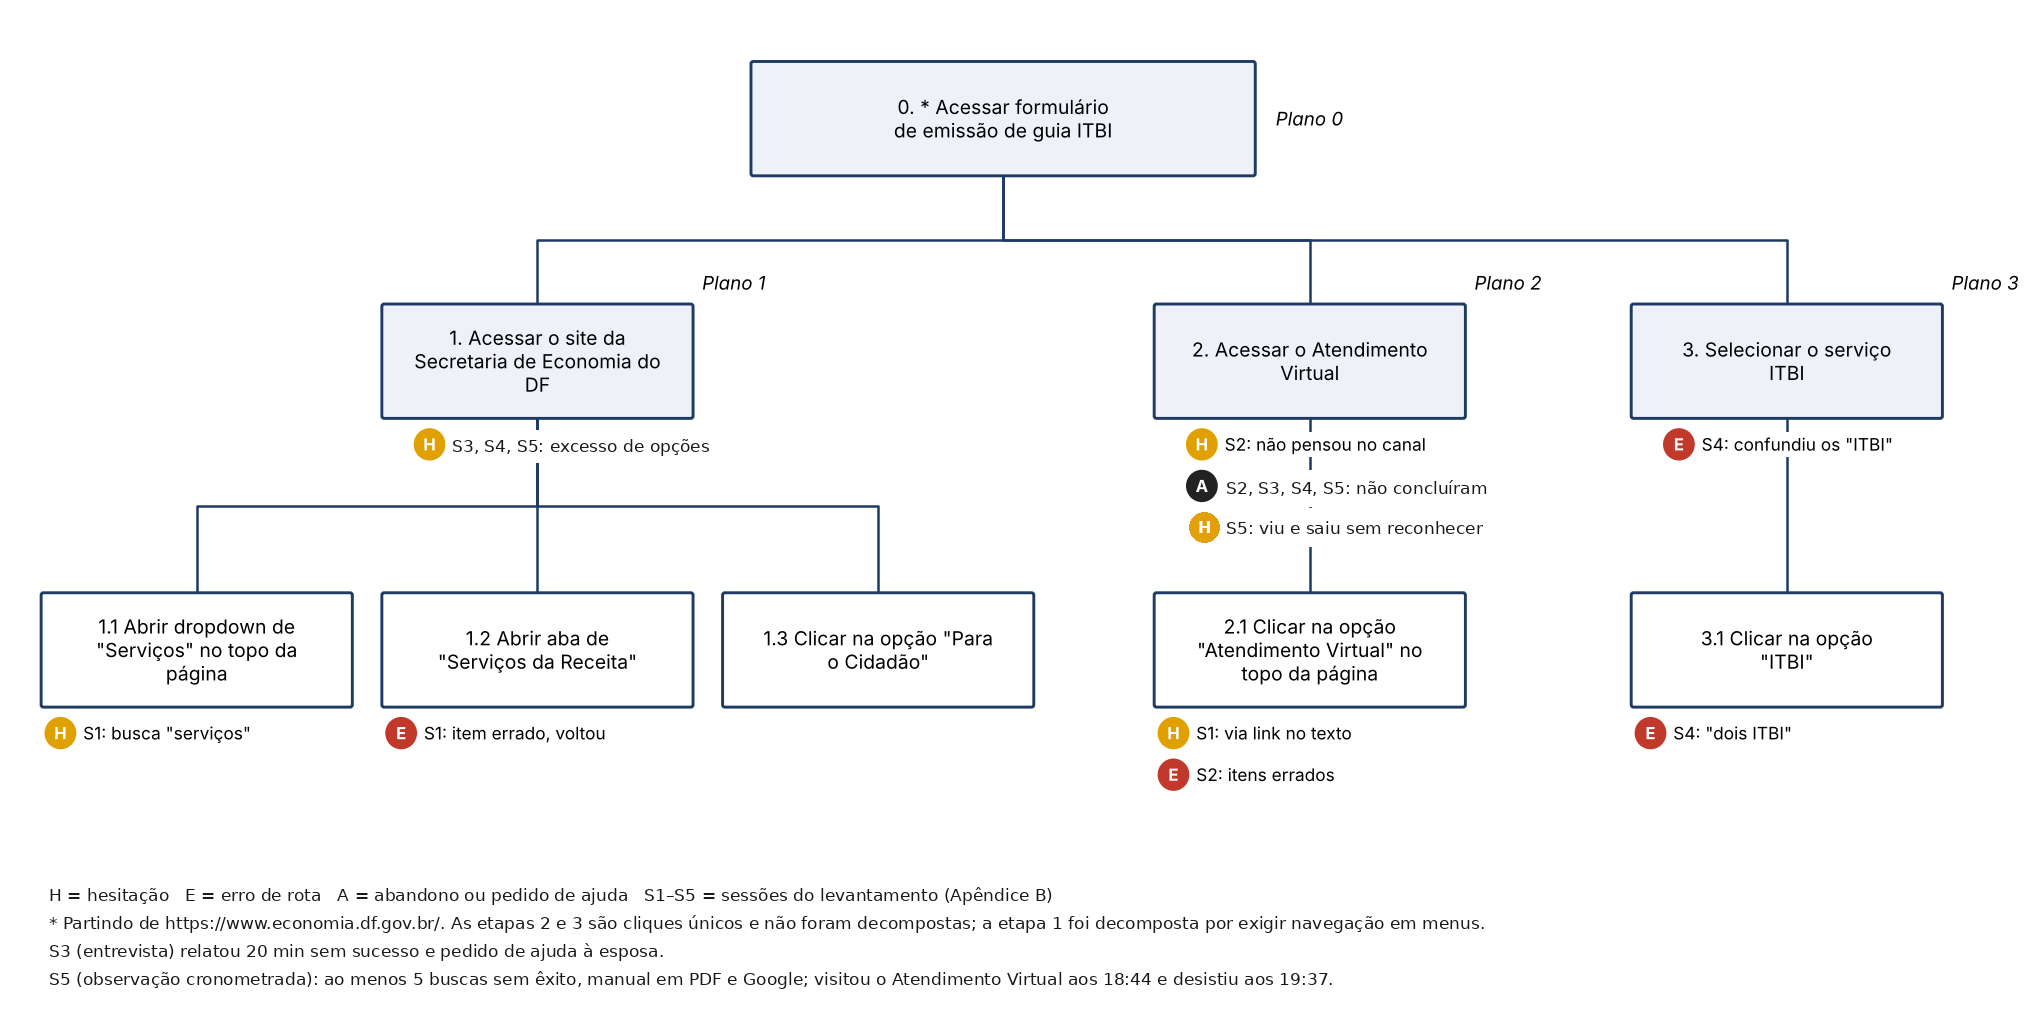
\includegraphics[width=0.97\textwidth,height=0.72\textheight,keepaspectratio]{figuras/hta.png}
  \fonte{Elaborada pelos autores com base em S1 a S5 (2026).}
\end{figure}
\end{landscape}

% =====================================================================
\chapter{Diagnóstico}\label{cap:diagnostico}
% =====================================================================

O diagnóstico reúne doze achados. Eles se apoiam em uma ou mais capturas de tela numeradas (Figuras~\ref{fig:achado1} a~\ref{fig:achado10}; os achados A11 e A12 remetem às telas já numeradas) e em um ou mais
princípios nomeados: \citeonline{norman2013} (golfos de execução e de avaliação,
significantes, mapeamento, \textit{feedback}, consistência, prevenção de erro,
reconhecimento em vez de recordação), as leis da Gestalt (proximidade,
similaridade, figura e fundo), a Lei de Fitts \cite{fitts1954} e a Lei de
Hick--Hyman \cite{hick1952}. Os achados vêm de inspeção heurística das cinco
telas e, quando há dado de sessão, da observação de uso (S1 a S5) e da inspeção complementar com NVDA e teclado; não houve
acesso a reclamações públicas nem a registros de ouvidoria. O
Quadro~\ref{qua:achados1} e o Quadro~\ref{qua:achados2} resumem os achados; a
discussão segue abaixo.

\fig[0.95]{achado1}{a1_menu.png}{Achado A1: menu Serviços com oito itens no primeiro nível e cinco no segundo, sem nenhum rótulo que nomeie a tarefa}{\capt{} (\texttt{economia.df.gov.br}).}

\textbf{A1. O menu Serviços lista categorias administrativas, e não tarefas.} O
menu abre à esquerda com Serviços da Receita, Reforma Tributária, Atendimento,
Sistemas, Serviços de TIC, Carta de Serviços, Ouvidoria e Escola de Governo e, no
segundo nível, Para o Cidadão, Para o Empresário, Outros Contribuintes, Governo e
Parceiros e Agendar Atendimento Presencial. Ninguém que procura ``emitir guia''
encontra essas palavras, e o item ``Atendimento'' (que abre um submenu) é
facilmente confundido com o Atendimento Virtual que se procura, que está em
outro lugar (S1 procurou ``Central de Atendimento ao Cidadão'', rolou a página e não achou nada).
Princípios: \textit{golfo de execução} de Norman (a pessoa sabe o que quer, mas
não sabe qual ação o sistema espera), Lei de Hick--Hyman (o tempo de decisão
cresce com o número de alternativas) e, como \textbf{hipótese ainda não
verificada}, a Lei de Fitts: o submenu só se mantém aberto se o ponteiro
percorre o trajeto na diagonal sem sair do item, comportamento que a captura estática não permite confirmar. Na inspeção por teclado, o problema é maior: o menu Serviços só se abre com o ponteiro (\textit{hover}); o submenu com Serviços da Receita e Para o Cidadão não abre com Tab, e o NVDA anuncia apenas ``Serviços, link'', sem informar que é um menu retrátil nem seu estado (achado A11).

\fig[0.95]{achado2}{c_cabecalhos.png}{Achado A2: três cabeçalhos, três identidades visuais e três domínios em um único fluxo}{\capt{} (cabeçalhos de \texttt{economia.df.gov.br}, \texttt{receita.fazenda.df.gov.br} e \texttt{atendimentovirtual.fazenda.df.gov.br}).}

\textbf{A2. O fluxo atravessa três sites que parecem três órgãos.} Muda o domínio,
o cabeçalho, a tipografia, a posição do ``Entrar'' (texto simples no portal,
botão escuro na Receita, campo CPF/CNPJ com dois botões claros no Atendimento
Virtual) e desaparece a barra ``Acessibilidade | Aa'', presente nos dois
primeiros. A pessoa que clica em um menu e cai em outro site perde a
referência de onde está. Princípios: consistência de Norman, \textit{feedback} de
localização e Gestalt de similaridade: elementos que devem agrupar-se como parte
do mesmo serviço não compartilham a mesma forma.

\fig[0.95]{achado3}{a3_catalogo.png}{Achado A3: catálogo da Receita para o item ITBI, com dez serviços nomeados pelo ato jurídico}{\capt{} (\texttt{receita.fazenda.df.gov.br}).}

\textbf{A3. O catálogo nomeia o ato, e não a tarefa.} O item ITBI reúne dez
serviços (Transmissão Onerosa -- Lançamento de ITBI; Cancelamento, Impugnação,
Prescrição e Restituição de ITBI; Demonstrativo de Cálculo e Termo de Quitação;
Imunidade e Isenção; Não Incidência; Efetuar Impugnação; Restituir ou Compensar;
Solicitar Cancelamento de Guia ou Declaração Eletrônica; Solicitar Prescrição de
Débitos). \textbf{Nenhum diz ``emitir guia''}, a ação que as cinco pessoas procuravam. A guia está atrás de ``Transmissão Onerosa -- Lançamento de ITBI'',
e S1 só o reconheceu ao ler a página (``Transmissão onerosa, lançamento de
ITBI. Acredito que seja essa opção''). S2 examinou, em voz alta, lançamento,
``segunda via'', ``cancelamento de guia'' e ``termos de quitação'' sem saber se
um deles era o procurado (``não é nenhum pouco intuitivo''). Princípios:
\textit{mapeamento} e golfo de execução (o vocabulário do sistema não mapeia o
vocabulário do usuário), \textit{reconhecimento em vez de recordação} (exige
conhecer o termo técnico) e Hick--Hyman (dez alternativas em duas colunas). O
impacto é maior nas personas 1, 2 e 4.

\fig[0.95]{achado4}{a4_contraste.png}{Achado A4: razões de contraste medidas nas capturas do catálogo e do formulário}{\capt{}; razões calculadas pelos autores com a fórmula da WCAG 2.2 \cite{wcag22}.}

\textbf{A4. O que indica o estado atual tem o menor contraste da tela.} Medidas
nas capturas, as razões são: categoria ITBI selecionada, 1,35:1; aba ativa
(``Para o Cidadão''), 1,69:1; título e faixa da página de serviço, 1,69:1;
abas inativas, 2,38:1; texto de ajuda do formulário, 2,61:1. O mínimo da
WCAG 2.2 é 4,5:1 para texto comum (critério 1.4.3) e 3:1 para componentes de
interface e estados (1.4.11). O item selecionado e a aba ativa, que deveriam
dizer ``você está aqui'', são \textbf{menos visíveis que os itens não
selecionados} e parecem desabilitados (a figura e o fundo se confundem). S1
disse, sem ser perguntada sobre cor, que o site é ``muito opaco'' e ``poderia ter
mais vida''. Princípios: \textit{feedback} e \textit{significante} de Norman
(o estado não é percebido), Gestalt de figura e fundo e, em acessibilidade,
1.4.3 e 1.4.11. As razões são preliminares e devem ser reconferidas com
ferramenta automática na inspeção (RA02 e RA03).

\fig[1.0]{achado5}{a5_faixa.png}{Achado A5: o caminho correto (Atendimento Virtual) é um entre quatro botões de mesmo peso, abaixo de um banner de maior destaque}{\capt{} (\texttt{receita.fazenda.df.gov.br}).}

\textbf{A5. A hierarquia visual do cabeçalho da Receita não aponta o caminho.}
O maior elemento é o banner de adesão à NFS-e, que não interessa a quem busca o
ITBI; abaixo, quatro botões idênticos (Serviços On-line, Agênci@net,
Atendimento Virtual, Legislação e Publicações) em MAIÚSCULAS, sem ícone, em
cinza escuro. O botão do qual depende a conclusão é um dos quatro e usa o
nome do canal. S2 registra a consequência: não pensou em ``Atendimento
Virtual'' para uma tarefa tributária, e S3 e S4 não chegaram a ele. Princípios:
Gestalt de similaridade e de proximidade (itens idênticos são lidos como
equivalentes), hierarquia visual e Hick--Hyman. O texto em maiúsculas também reduz a legibilidade em frases mais longas. S5 confirma o efeito no extremo: visitou o Atendimento Virtual aos 18 min 44 s e saiu em poucos segundos, sem identificar que era o que procurava.

\fig[0.95]{achado6}{c_itbi.png}{Achado A6: ``ITBI'' designa o item do catálogo, o cartão do Atendimento Virtual e o assunto do formulário}{\capt{} (\texttt{receita.fazenda.df.gov.br} e \texttt{atendimentovirtual.fazenda.df.gov.br}).}

\textbf{A6. O mesmo rótulo designa três coisas diferentes.} ``ITBI'' é, no nível 1,
a categoria do catálogo da Receita (que leva a dez serviços); no nível 2, o cartão
do Atendimento Virtual (que leva ao formulário); e, no nível 3, o assunto
dentro do formulário. S4 disse não entender ``por que existia duas abas
diferentes com o mesmo nome, sendo que uma é muito mais simples e faz muito mais
sentido''. Além disso, os cartões ITBI e ITCD têm a sigla como único texto (``ITCD''
nem é expandida), exigindo recordação do que significam. Princípios:
\textit{modelo conceitual} e consistência de Norman (um nome, um referente),
\textit{reconhecimento em vez de recordação} e, no caso das siglas, o uso de
termo técnico sem tradução, que pesa mais para a persona 4. Em S5 a sigla também foi um obstáculo: o participante interrompeu a busca para perguntar o que significa ITBI. Na inspeção com NVDA, ITBI e ITCD são lidas letra por letra, sem expansão (\textit{abbr}) ou alternativa, e os cartões são imagens com o texto embutido e sem texto alternativo (RA10).

\fig[0.95]{achado7}{a7_busca.png}{Achado A7: duas buscas disponíveis (Receita e Atendimento Virtual), ignoradas em S1 a S4 e sem êxito em S5}{\capt{}.}

\textbf{A7. A busca existe, é pouco usada e, quando usada, não leva ao formulário.}
O portal da Receita oferece o campo ``O que você procura? Ex.: Segunda via
IPVA'' e o Atendimento Virtual oferece ``Procure aqui o atendimento desejado''.
Em S1 a S4, \textbf{nenhum participante cita ou usa a busca}; todos navegaram por
menus e cartões, e o roteiro não perguntou por quê. Em S5 foi o contrário: a busca
foi o primeiro reflexo (``instinto primário''), repetida ao menos cinco vezes em
sites diferentes (00:00, 00:33, 02:10, 11:32 e 19:00), e \textbf{sempre devolveu
conteúdo relacionado ao ITBI (manuais e requerimentos em PDF), nunca o formulário}.
O participante perguntou duas vezes se ``a barra de pesquisa não funciona'', abriu
o manual, recorreu a \textit{Ctrl+F} dentro do PDF, baixou requerimentos,
pesquisou no Google e acabou desistindo aos 19 min 37 s. A desorientação foi tamanha
que a busca interna de um PDF e a busca externa foram mais usadas que a navegação
do próprio portal. Princípios: \textit{significante} (a busca não se anuncia como
atalho para quem não a tentou), \textit{mapeamento} e golfo de avaliação (o
resultado não corresponde à intenção ``emitir guia'', e o usuário não sabe se errou
a consulta ou se a busca falha) e Hick--Hyman (uma busca eficaz trocaria N
alternativas por um campo). A hipótese para S1 a S4 é baixa descoberta (o campo da
Receita fica abaixo do banner e dos quatro botões); a de S5, baixa precisão. Ambas
devem ser testadas na Entrega~2.

\fig[0.95]{achado8}{a8_login.png}{Achado A8: o aviso de login aparece só no Atendimento Virtual, entre seis botões de ação e uma busca}{\capt{} (\texttt{atendimentovirtual.fazenda.df.gov.br}).}

\textbf{A8. As exigências do serviço só aparecem no fim.} O aviso ``Efetue o
LOGIN para ter acesso a todos os serviços'' só aparece na etapa 2, depois de duas
ou três páginas. S1 só soube que precisava de CPF e senha no último passo (``aí vai pedir
o CPF e senha''), e S1 e S4 não sabiam quais documentos levar e descobriram
perguntando a atendentes. Existe um botão ``Passo a Passo'', mas ele é o sexto de
seis verbos com o mesmo peso (Registrar Solicitação, Consultar, Reabrir,
Complementar, Avaliar, Passo a Passo). Princípios: \textit{feedback} e
visibilidade do estado do sistema (o usuário não sabe o que vem), golfo de
avaliação e prevenção de erro (informar o pré-requisito antes de o usuário
investir tempo). É o achado que mais pesa para quem tem pouco tempo, ou seja,
as personas 1, 3 e 6. Na inspeção com NVDA, o aviso de login passa despercebido se a pessoa salta direto ao campo de busca por atalho de teclado.

\fig[0.78]{achado9}{a9_form.png}{Achado A9: formulário com dois seletores dependentes, asterisco claro de obrigatoriedade e editor de texto com mais de uma dezena de botões}{\capt{} (\texttt{atendimentovirtual.fazenda.df.gov.br}).}

\textbf{A9. O formulário pede decisões que o usuário não consegue tomar com
segurança.} Depois de Assunto = ITBI (com uma marca verde ambígua: confirma a
escolha ou indica sucesso do envio?), o campo Tipo de Atendimento volta a pedir
``Selecione'', e S1 precisou escolher ``emitir guia de ITBI serviço'' em uma lista
sem pré-seleção. Obrigatório é indicado por um asterisco vermelho claro,
quase invisível; ``Selecione o tipo de documento do usuário'' tem três botões de
opção sem marca de obrigatoriedade e a Descrição abre um editor de texto com
mais de uma dezena de botões, vários de ícone, entre eles ``</>'' e ``?'', sem rótulo, para uma
solicitação de uma linha. O texto de ajuda, em azul claro, mede 2,61:1.
Princípios: Hick--Hyman (muitos controles), \textit{significantes} e
\textit{restrições} de Norman (o ícone não diz o que faz; a obrigatoriedade
não é percebida), \textit{prevenção de erro} e, em acessibilidade, 3.3.2 e 1.4.3. Na inspeção por teclado, o foco \textbf{fica preso} no editor da Descrição (Tab e Shift+Tab não saem dele), o que viola o critério 2.1.2, e a barra de formatação exige dezenas de toques de Tab antes de chegar à área de digitação. O NVDA lê os ícones como ``Botão'', sem nome, e o asterisco de obrigatoriedade não está associado programaticamente ao campo (sem \texttt{aria-required}): ``E-mail, edição, em branco'' não avisa que o preenchimento é obrigatório.

\fig[0.7]{achado10}{c_governo.png}{Achado A10: ``Governo e Parceiros'' no menu e ``Governos e Parceiros'' na aba}{\capt{}.}

\textbf{A10. O mesmo item tem dois nomes.} O menu do portal chama o destino de
``Governo e Parceiros''; a aba equivalente na Receita, ``Governos e
Parceiros''. A diferença é pequena (um \textit{s}) e a consequência também, mas
indica ausência de um vocabulário controlado, a mesma causa raiz dos achados A3
e A6. Princípios: consistência e padronização de Norman, e o critério 3.2.4 da WCAG
(identificação consistente).

\textbf{A11. O fluxo previsto não pode ser percorrido por teclado nem lido com
confiança por leitor de tela.} A inspeção complementar com NVDA e teclado
(seção~2.3) mostrou: (i) no portal institucional, o submenu
Serviços não abre com Tab, porque só reage a \textit{hover} e não tem
\texttt{aria-expanded}, e o topo e a navegação não têm regiões semânticas
(\texttt{nav}, \texttt{header}); (ii) no catálogo da Receita, o indicador de foco
tem baixo contraste ou foi removido na faixa de botões e nos itens, o foco passa
pelo campo de busca antes dos botões principais e a lista em três colunas é lida
como blocos soltos, sem hierarquia nem contagem; (iii) no Atendimento Virtual, os
cartões são imagens com texto embutido, sem texto alternativo, em
\texttt{div} sem \texttt{tabindex} nem \texttt{role="button"}, de modo que Tab os
salta e a pessoa não consegue selecionar o ITBI; (iv) no formulário, o editor de
texto prende o foco. Em consequência, as etapas 1.1, 2.1 e 3.1 da HTA são
inoperantes para quem não usa mouse. Princípios: \textit{restrições} e
mapeamento de Norman (o ponteiro é o único modo de operar) e \textit{prevenção de
erro}; na WCAG, 1.3.1, 2.1.1, 2.1.2, 2.4.3, 2.4.7 e 4.1.2. Evidência: as telas das
Figuras~\ref{fig:achado1}, \ref{fig:achado6} e~\ref{fig:achado9}. Como a inspeção
foi feita por integrante sem deficiência visual, o achado indica falha técnica e
não mede a dificuldade real de quem usa leitor de tela, o que depende de teste com
essas pessoas (limitação (vi), seção~\ref{sec:limitacoes}).

\textbf{A12. A interface não se adapta a 320 px e há alvos menores que o mínimo.} Na simulação responsiva com o \textit{viewport} do navegador ajustado para 320 px, condição equivalente a zoom de 400\% em uma janela inicial de 1280 px, observou-se rolagem horizontal bidirecional nas tabelas, nos formulários legados e no cabeçalho estático, além de sobreposição de texto nos menus secundários. Na medição manual das dimensões dos alvos interativos no inspetor de elementos do navegador, ficaram abaixo de 24\,$\times$\,24 px os links secundários do catálogo da Receita, os ícones de ação e a paginação nos cartões do Atendimento Virtual e os botões de fonte e contraste no topo do portal. Princípios: Lei de Fitts e critérios 1.4.10 (refluxo) e 2.5.8 (tamanho do alvo) da WCAG 2.2. A simulação e as medições confirmam barreiras técnicas, mas não substituem a avaliação com usuários. Evidência: Figuras~\ref{fig:achado1}, \ref{fig:achado2}, \ref{fig:achado3}, \ref{fig:achado5}, \ref{fig:achado8} e~\ref{fig:achado9}.

\begin{landscape}
\begin{quadro}[!htbp]
  \caption{Achados do diagnóstico (A1 a A5)}\label{qua:achados1}
  \centering\footnotesize
  \begin{tabularx}{\linewidth}{|c|Y|c|p{3.2cm}|p{4.2cm}|Y|}\hline
    \textbf{ID} & \textbf{Achado} & \textbf{Evidência} & \textbf{Origem} & \textbf{Princípio(s) violado(s)} & \textbf{Impacto nas personas} \\\hline
    A1 & Menu Serviços organizado por categoria administrativa, sem rótulo de tarefa; ``Atendimento'' confundível com Atendimento Virtual; submenu só abre por \textit{hover} & Fig.~\ref{fig:achado1} & Inspeção heurística rápida; observação S1; inspeção por teclado e NVDA & Norman: golfo de execução; Lei de Hick--Hyman; Lei de Fitts (hipótese); WCAG 2.1.1 & Persona 3 hesita e erra; personas 1 e 4 se perdem no excesso de itens \\\hline
    A2 & Três subdomínios com cabeçalho, ``Entrar'' e barra de acessibilidade diferentes & Fig.~\ref{fig:achado2} & Inspeção heurística rápida & Norman: consistência e \textit{feedback} de localização; Gestalt: similaridade & Personas 1, 3 e 6 perdem a referência de lugar; persona 5 relê cabeçalhos diferentes a cada site \\\hline
    A3 & Catálogo de ITBI com dez itens nomeados pelo ato jurídico; nenhum diz ``emitir guia'' & Fig.~\ref{fig:achado3} & Observação S1, S2, S3 e S4; inspeção heurística & Norman: mapeamento, golfo de execução, reconhecimento em vez de recordação; Hick--Hyman & Maior impacto nas personas 1, 2 e 4 (vocabulário jurídico) \\\hline
    A4 & Contraste de 1,35:1 a 2,61:1 em estado selecionado, abas, títulos e texto de ajuda & Fig.~\ref{fig:achado4} & Inspeção própria (medição); fala de S1 (``muito opaco'') & Norman: \textit{feedback}, significante; Gestalt: figura e fundo; WCAG 1.4.3 e 1.4.11 & Personas 1 e 5 (baixa visão, idade); todas em tela com brilho baixo ou ao sol \\\hline
    A5 & Botão ``Atendimento Virtual'' é um de quatro de mesmo peso, abaixo do banner NFS-e & Fig.~\ref{fig:achado5} & Observação S2, S3, S4 e S5; inspeção heurística & Gestalt: similaridade e proximidade; hierarquia visual; Hick--Hyman & Personas 1, 2, 4 e 7 não percebem a rota correta (S5 a visitou e saiu) \\\hline
  \end{tabularx}
  \fonte{Elaborado pelos autores (2026).}
\end{quadro}
\end{landscape}

\begin{landscape}
\begin{quadro}[!htbp]
  \caption{Achados do diagnóstico (A6 a A12)}\label{qua:achados2}
  \centering\footnotesize
  \begin{tabularx}{\linewidth}{|c|Y|c|p{3.2cm}|p{4.2cm}|Y|}\hline
    \textbf{ID} & \textbf{Achado} & \textbf{Evidência} & \textbf{Origem} & \textbf{Princípio(s) violado(s)} & \textbf{Impacto nas personas} \\\hline
    A6 & ``ITBI'' designa a categoria do catálogo, o cartão do Atendimento Virtual e o assunto do formulário; siglas sem expansão; cartões sem texto alternativo & Fig.~\ref{fig:achado6} & Observação S4 e S5; inspeção heurística e NVDA & Norman: modelo conceitual, consistência, reconhecimento em vez de recordação & Persona 2 errou de ``ITBI''; persona 4 sem repertório para as siglas \\\hline
    A7 & Duas buscas disponíveis: ignoradas em S1 a S4; em S5, usadas ao menos cinco vezes sem chegar ao formulário & Fig.~\ref{fig:achado7} & Observação S1 a S5; inspeção heurística & Norman: significante; Hick--Hyman (busca como atalho) & Persona 7 desistiu depois de cinco buscas; todas as demais ganhariam com uma busca eficaz; a persona 6 pagaria menos cargas de página \\\hline
    A8 & Login e documentos só são informados ao final; ``Passo a Passo'' é um entre seis botões iguais & Fig.~\ref{fig:achado8} & Observação S1 e S4; inspeção heurística e NVDA & Norman: \textit{feedback}, golfo de avaliação, prevenção de erro & Personas 1, 3 e 6 gastam tempo e franquia antes de saber o que falta \\\hline
    A9 & Formulário com seletor dependente, obrigatoriedade pouco visível, ícones sem nome e editor de texto rico que prende o foco do teclado & Fig.~\ref{fig:achado9} & Inspeção heurística; observação S1; inspeção por teclado e NVDA & Hick--Hyman; Norman: significante e restrição; prevenção de erro; WCAG 3.3.2, 1.4.3, 2.1.2, 4.1.2 & Personas 4 e 5 (leitor de tela lê ícones sem nome); persona 2 em tela pequena \\\hline
    A10 & ``Governo e Parceiros'' (menu) versus ``Governos e Parceiros'' (aba) & Fig.~\ref{fig:achado10} & Inspeção heurística; benchmarking com padrão (DSGov) & Norman: consistência; WCAG 3.2.4 & Efeito pequeno isolado; sintoma de vocabulário não controlado (A3, A6) \\\hline
    A11 & Menu, cartões e editor do formulário não operáveis por teclado; foco, nomes e regiões ausentes para o leitor de tela & Figs.~\ref{fig:achado1}, \ref{fig:achado6} e~\ref{fig:achado9} & Inspeção própria (NVDA e teclado) & Norman: restrições, mapeamento; WCAG 1.3.1, 2.1.1, 2.1.2, 2.4.3, 2.4.7, 4.1.2 & Persona 5 não completa o fluxo; quem não usa mouse, por qualquer motivo, fica bloqueado (hipótese a validar) \\\hline
    A12 & Refluxo inadequado a 320 px e alvos menores que 24 por 24 px & Figs.~\ref{fig:achado1}, \ref{fig:achado2}, \ref{fig:achado3}, \ref{fig:achado5}, \ref{fig:achado8} e~\ref{fig:achado9} & Simulação responsiva; medição manual no inspetor do navegador & WCAG 1.4.10 e 2.5.8; Lei de Fitts & Persona 2 (Júlia, celular): barreiras confirmadas por inspeção; persona 6: reforça hipótese de dificuldade em tela pequena \\\hline
  \end{tabularx}
  \fonte{Elaborado pelos autores (2026).}
\end{quadro}
\end{landscape}



\textbf{Síntese: uma causa raiz.} Seis dos doze achados (A1, A3, A5, A6, A7 e A10) partilham uma causa: \textbf{o vocabulário do portal é do órgão, e não do
cidadão}, e o site é organizado por canal (Atendimento Virtual, Agênci@net) e
por ato jurídico (lançamento, impugnação), enquanto o usuário organiza o mundo
por tarefa (``emitir a guia''). É o que o enunciado chama de golfo de execução, e
o que S2 sugeriu, ao propor que as ``palavras-chave das coisas que as pessoas
mais usam'' aparecessem já no menu. A consequência para as Entregas 2 e 3 é que
as correções de maior retorno são lexicais e estruturais (nomear a tarefa,
expor a busca, informar pré-requisitos), antes das visuais.

% =====================================================================
\chapter{Padronização e estilos de interação}\label{cap:padronizacao}
% =====================================================================

\section{Inconsistências internas}\label{sec:padr-int}

Três comparações lado a lado já foram apresentadas como evidência de
diagnóstico e são retomadas aqui sob o ângulo da padronização.

\begin{itemize}
  \item \textbf{Cabeçalho e conta} (Figura~\ref{fig:achado2}). A ação ``Entrar''
    tem três formas (texto, botão-pílula escuro, campo com dois botões claros) e
    posições diferentes; a barra de acessibilidade, que existe nos dois primeiros
    sites, não existe no terceiro, que é onde está o formulário. Uma
    ferramenta de acessibilidade presente em dois terços do fluxo e ausente
    exatamente onde a pessoa preenche dados é uma inconsistência funcional, e
    não apenas estética.
  \item \textbf{Mesmo rótulo, referentes diferentes} (Figura~\ref{fig:achado6}). Os
    três ``ITBI'' têm três aparências: linha de lista cinza, cartão azul com
    ícone, seletor de formulário. A recomendação de Norman é que um mesmo nome
    aponte para o mesmo conceito; aqui aponta para três.
  \item \textbf{Mesmo destino, dois nomes} (Figura~\ref{fig:achado10}).
    ``Governo e Parceiros'' e ``Governos e Parceiros''.
\end{itemize}

Há ainda uma inconsistência de \textbf{estado}: o item ativo da lista e a aba ativa
são os de menor contraste (Figura~\ref{fig:achado4}), o oposto do que a
convenção de interfaces estabelece (o ativo se destaca do inativo).

\section{Aderência ao DSGov}

A comparação é visual e qualitativa, feita com os princípios gerais do Padrão
Digital de Governo \cite{dsgov} e com a Aula 2 da disciplina
\cite{aulaprincipios}; não se inspecionou o código para identificar os
componentes do DSGov e a lista de tokens não foi usada como \textit{checklist}.
Por isso as conclusões abaixo são de desvio aparente em relação aos princípios do
padrão (consistência, contraste conforme a WCAG, rótulos e \textit{feedback}),
e não de não conformidade formal.

\begin{quadro}[!htbp]
  \caption{Aderência do fluxo aos princípios do DSGov}\label{qua:dsgov}
  \centering\small
  \begin{tabularx}{\textwidth}{|l|Y|Y|}\hline
    \textbf{Elemento} & \textbf{Esperado pelo padrão (princípio)} & \textbf{Observado no fluxo} \\\hline
    Cabeçalho e identidade & Estrutura única de cabeçalho em todo o serviço, com barra de acessibilidade & Três cabeçalhos; barra de acessibilidade ausente no Atendimento Virtual (A2) \\\hline
    Menu & Itens que descrevem destinos de forma consistente & Itens por canal e por categoria; ``Atendimento'' e ``Atendimento Virtual'' coexistem (A1, A5) \\\hline
    Abas e estado ativo & Estado ativo distinguível, com contraste suficiente & Aba ativa e item ativo com 1,69:1 e 1,35:1 (A4) \\\hline
    Cores e contraste & Combinações que atendam o nível AA & Pares abaixo de 3:1 em texto e em estado (A4, A9) \\\hline
    Busca & Campo de busca visível e funcional como atalho & Existe, em duas versões diferentes; ignorado em S1 a S4 e sem êxito em S5 (A7) \\\hline
    Formulário & Rótulo visível, indicação clara de obrigatoriedade, ajuda legível & Rótulo visível, mas asterisco claro, ajuda a 2,61:1, ícones sem rótulo (A9) \\\hline
    Mensagens e \textit{feedback} & Aviso de pré-requisito antes da ação & Login informado só no Atendimento Virtual (A8) \\\hline
    Vocabulário & Termos controlados e na linguagem do cidadão & Termos jurídicos e três referentes para ``ITBI'' (A3, A6, A10) \\\hline
  \end{tabularx}
  \fonte{Elaborado pelos autores com base em \citeonline{dsgov} (2026).}
\end{quadro}

Em chave de \textit{benchmarking}, S2 comparou o site com o portal do governo
federal: ``as funcionalidades são bem óbvias, tem palavras-chave bem mais fáceis
de achar'', enquanto no do GDF ``é como se tivesse escondida''. Trata-se de
percepção de uma participante, não de medição, mas converge com A3 e A7.

\section{Estilos de interação}

\begin{quadro}[!htbp]
  \caption{Estilos de interação presentes e adequação às personas}\label{qua:estilos}
  \centering\small
  \begin{tabularx}{\textwidth}{|l|Y|Y|}\hline
    \textbf{Estilo} & \textbf{Onde aparece} & \textbf{Adequação às personas} \\\hline
    Menu em cascata (\textit{dropdown}) & Portal institucional (Serviços, dois níveis) & Exige precisão de ponteiro e conhecimento prévio da categoria; inadequado para as personas 1 e 4; não abre por teclado, o que bloqueia a persona 5 (A11, RA05) \\\hline
    Navegação por catálogo (lista em três colunas) & Receita (Para o Cidadão) & Funciona para quem reconhece o termo jurídico (persona 3); exige recordação para as personas 2 e 4 \\\hline
    Seleção por cartões com ícone & Atendimento Virtual (cartões de serviço) & Reconhecimento visual ajuda a persona 4, mas o texto fica embutido na imagem, a sigla não se explica (A6) e os cartões não recebem foco por teclado (A11) \\\hline
    Busca por palavra-chave & Receita e Atendimento Virtual & Seria o estilo mais adequado às personas 1, 2, 4, 6 e 7 se funcionasse com o vocabulário do cidadão; hoje é pouco perceptível e, quando usado (S5), devolve manuais e requerimentos e não o formulário (A7) \\\hline
    Preenchimento de formulário & Atendimento Virtual & Longo e com editor de texto rico; custoso para as personas 1, 4 e 6; ícones sem rótulo para a persona 5 (A9) \\\hline
    Ajuda passo a passo & Atendimento Virtual (``Passo a Passo'') & Estilo adequado a todas as classes, mas está escondido entre seis botões (A8) \\\hline
  \end{tabularx}
  \fonte{Elaborado pelos autores (2026).}
\end{quadro}

% =====================================================================
\chapter{Requisitos de usabilidade}\label{cap:requisitos}
% =====================================================================

\section{Classes de contexto}

\begin{quadro}[!htbp]
  \caption{Classes de contexto}\label{qua:classes}
  \centering\small
  \begin{tabularx}{\textwidth}{|l|Y|l|}\hline
    \textbf{Classe} & \textbf{Caracterização (origem no levantamento)} & \textbf{Personas} \\\hline
    C1 --- Familiarizado com a web & Declara-se acostumado à web, usa menus e links com autonomia e se recupera de erros por navegação lateral ou por busca externa; ainda assim falhou, desistiu ou precisou de várias tentativas (S1, S2, S5). Pode ser eventual no serviço, e é recorrente na web. & 3 e 7 \\\hline
    C2 --- Eventual com baixo letramento digital & Depende de apoio de terceiros para navegar; desiste cedo e se perde no excesso de opções e no vocabulário técnico (S3); inclui, por hipótese, pessoas de baixa escolaridade (persona 4, fontes secundárias). & 1 e 4 \\\hline
    C3 --- Acesso ou percepção restrita & Usa celular como dispositivo principal (S4), tem conexão ou aparelho limitados, ou depende de leitor de tela ou de ampliação (hipóteses de base secundária). & 2, 5 e 6 \\\hline
  \end{tabularx}
  \fonte{Elaborado pelos autores com base em S1 a S5, \citeonline{ticdomicilios} e \citeonline{webaim2024} (2026).}
\end{quadro}

\section{Requisitos}

Os requisitos seguem o modelo de meta de cinco partes do material da disciplina
\cite{aulatema7}: dimensão, contexto, métrica, alvo e verificação. Para cada
alvo, adotam-se dois patamares: o \textbf{alvo planejado} e o \textbf{pior caso
aceitável}.

\textbf{Regra de veredito.} Para as métricas de proporção (RU01 a RU06), a
verificação compara o limite inferior unilateral de 95\% do intervalo de
Clopper--Pearson \cite{clopper1934} com os patamares: \textit{atende} se o
limite inferior alcança o alvo planejado; \textit{atende ao mínimo} se alcança
o pior caso aceitável; \textit{não atende} se o limite superior fica abaixo do
pior caso; \textit{inconclusivo} nos demais. A regra é conservadora com amostras
pequenas: com $n=8$, mesmo 8 sucessos em 8 só confirmam 68,8\%, e com
$n=10$ nove sucessos já confirmam 60,6\% e dez, 74,1\%. Por isso se fixa
$n=10$ por classe, e com $n$ menor o resultado será, quando muito, indicativo.
Para a satisfação (RU07 e RU08), compara-se o limite inferior do intervalo de
confiança de 95\% da média do SUS \cite{brooke1996,sauro2016}. Cada
requisito de tempo ou de erro é pareado com um de eficácia na mesma classe
(RU04 com RU01; RU05 e RU06 com RU02), para que o tempo só conte quando a tarefa
foi concluída, evitando otimizar uma métrica à custa da outra.

\textbf{Âncora de satisfação.} O padrão oficial de qualidade é nota média de
4,5 em 5 \cite{padroesqualidade}. Adotou-se a conversão linear
$\mathrm{nota}=1+4\times\mathrm{SUS}/100$, na qual 4,5 corresponde a SUS $=87{,}5$.
O pior caso aceitável é o SUS 68, média de referência da escala
\cite{sauro2016}. A conversão é uma escolha da equipe e deve ser confirmada com a
professora.

\textbf{Tempos e erros.} O roteiro não perguntou aos participantes quanto tempo ou
quantas tentativas consideram aceitável (seção~\ref{cap:levantamento}, item (e)).
Os alvos de tempo e de erro assumem, por isso, uma meta baseada na frustração
observada: embora não questionados, os participantes demonstraram exaustão ou
desistência em tempos totais de sessão de 7 a quase 20 minutos de uso ineficaz
(S5: 19 min 37 s). Com essa observação e a premissa de um serviço público digital
rápido, a equipe fixou o alvo hipotético de \textbf{conclusão em até 5 minutos} e a
tolerância de \textbf{no máximo 1 erro de rota}; o limite inaceitável é o de 7
minutos, menor tempo total de sessão registrado entre os que terminaram sem êxito
ou com ajuda de terceiros (S3). São hipóteses a validar na Entrega~3.

\requisito{RU01}{Eficácia}{Etapas 1 a 3 da HTA (objetivo 0)}{C1: familiarizado com a web}%
  {Proporção de participantes que chegam ao formulário com Assunto = ITBI sem ajuda de terceiros e sem intervenção do moderador.}%
  {Planejado: $\geq$ 80\% dos participantes. Pior caso aceitável: $\geq$ 60\%. Linha de base observada: 1 de 3 (S1 sim; S2 e S5 não); sem valor inferencial.}%
  {Contagem de sucesso e falha em teste moderado, $n=10$; veredito pelo limite inferior de Clopper--Pearson.}

\requisito{RU02}{Eficácia}{Etapas 1 a 3 da HTA (objetivo 0)}{C2: eventual com baixo letramento digital}%
  {Proporção de participantes que chegam ao formulário com Assunto = ITBI sem ajuda de terceiros e sem intervenção do moderador.}%
  {Planejado: $\geq$ 80\% dos participantes. Pior caso aceitável: $\geq$ 60\%. Linha de base: 0 de 1 (S3, relato).}%
  {Contagem de sucesso e falha em teste moderado, $n=10$; veredito pelo limite inferior de Clopper--Pearson.}

\requisito{RU03}{Eficácia}{Etapas 1 a 3 da HTA (objetivo 0), em celular}{C3: acesso ou percepção restrita}%
  {Proporção de participantes que chegam ao formulário com Assunto = ITBI sem ajuda de terceiros, usando celular em tela de até 412 px de largura.}%
  {Planejado: $\geq$ 80\% dos participantes. Pior caso aceitável: $\geq$ 60\%. Linha de base: 0 de 1 (S4).}%
  {Contagem de sucesso e falha em teste moderado, $n=10$; veredito pelo limite inferior de Clopper--Pearson. O uso com leitor de tela é verificado nos RA, e não neste requisito.}

\requisito{RU04}{Eficiência}{Etapas 1 a 3 da HTA (objetivo 0)}{C1: familiarizado com a web}%
  {Proporção de participantes que concluem o fluxo, do carregamento da página inicial à exibição do formulário, dentro do tempo-limite.}%
  {Planejado: $\geq$ 80\% em até 5 minutos. Pior caso aceitável: $\geq$ 60\% em até 7 minutos. Linha de base: S5 desistiu em 19 min 37 s; S1 e S2 usaram 10 e 9 minutos de sessão.}%
  {Cronometragem em teste moderado, $n=10$, contando apenas as execuções concluídas sem ajuda (par de RU01).}

\requisito{RU05}{Eficiência}{Etapas 1 a 3 da HTA (objetivo 0)}{C2: eventual com baixo letramento digital}%
  {Proporção de participantes que concluem o fluxo, do carregamento da página inicial à exibição do formulário, dentro do tempo-limite.}%
  {Planejado: $\geq$ 80\% em até 5 minutos. Pior caso aceitável: $\geq$ 60\% em até 7 minutos. Linha de base: S3 chamou ajuda em sessão de 7 minutos e relatou cerca de 20 minutos na tentativa.}%
  {Cronometragem em teste moderado, $n=10$, contando apenas as execuções concluídas sem ajuda (par de RU02).}

\requisito{RU06}{Eficiência}{Subtarefas 1.1, 1.2, 1.3 e 2.1 da HTA}{C2: eventual com baixo letramento digital}%
  {Proporção de participantes que cometem no máximo um erro de rota (clique em item que não leva ao formulário, seguido de retorno).}%
  {Planejado: $\geq$ 80\% com no máximo 1 erro de rota (tolerância fixada pela equipe). Pior caso aceitável: $\geq$ 60\% com no máximo 2. Linha de base: S2, ao menos 3; S1, ao menos 1; S4, ao menos 1; S5, vários (cinco buscas e três sites).}%
  {Contagem de erros em teste moderado, $n=10$, sobre a gravação das ações (par de RU02).}

\requisito{RU07}{Satisfação}{Fluxo completo (objetivo 0)}{C1: familiarizado com a web}%
  {Escore SUS médio, após a tarefa.}%
  {Planejado: média $\geq$ 87,5 (equivale a 4,5 em 5 pela conversão linear). Pior caso aceitável: limite inferior do IC de 95\% $\geq$ 68.}%
  {Escala SUS aplicada após teste moderado, $n=10$.}

\requisito{RU08}{Satisfação}{Fluxo completo (objetivo 0)}{C2: eventual com baixo letramento digital}%
  {Escore SUS médio, após a tarefa.}%
  {Planejado: média $\geq$ 87,5 (equivale a 4,5 em 5 pela conversão linear). Pior caso aceitável: limite inferior do IC de 95\% $\geq$ 68. A meta é a mesma de RU07: não se admite satisfação menor para quem tem menos letramento.}%
  {Escala SUS aplicada após teste moderado, $n=10$.}

\textbf{Cobertura.} Três requisitos de eficácia, três de eficiência e dois de
satisfação, no total de oito. A classe C3 tem requisito de eficácia (RU03) e
tem, de resto, cobertura dos requisitos de acessibilidade, porque é a classe
cujos principais obstáculos (leitor de tela, tela pequena, contraste) são
verificáveis por inspeção. A ausência de RU de eficiência e satisfação para C3 é
consciente: com no máximo oito requisitos, priorizou-se a classe com a falha
observada mais clara (C2) e a classe com o dado mais favorável (C1), que fixa o
teto do que é possível.

% =====================================================================
\chapter{Requisitos de acessibilidade}\label{cap:acessibilidade}
% =====================================================================

Em atendimento ao art.~63 da Lei n.º 13.146/2015 \cite{lbi2015} e ao padrão de
conformidade de acessibilidade da administração pública \cite{emag}, adota-se o
nível de conformidade \textbf{AA} da WCAG 2.2 \cite{wcag22}. A verificação
ocorre por inspeção (ferramenta automática e navegação manual por teclado e
leitor de tela). Os doze critérios abaixo foram escolhidos por serem aplicáveis
ao fluxo e por haver indício, nas capturas ou nas sessões, de risco de falha.

A equipe realizou a inspeção própria complementar descrita na seção~2.3: leitor de
tela NVDA (modos de navegação e de foco), navegação exclusiva por teclado (Tab,
Shift+Tab, Enter, Espaço e setas), medição de contraste, simulação responsiva a
320 px e medição do tamanho dos alvos. \textbf{Os doze requisitos foram verificados
e nenhum é atendido pelo serviço atual.} A simulação de refluxo foi feita no modo
responsivo das ferramentas de desenvolvedor do navegador, com \textit{viewport} de
320 px (equivalente a zoom de 400\% em janela inicial de 1280 px); os alvos foram
medidos manualmente pelo inspetor de elementos do navegador. A inspeção com NVDA e
teclado foi feita por integrante sem deficiência visual e, por isso, simula, mas
não substitui, o uso por pessoa usuária de leitor de tela.

\begin{quadro}[!htbp]
  \caption{Requisitos de acessibilidade e resultado da inspeção}\label{qua:ra}
  \centering\scriptsize
  \begin{tabularx}{\textwidth}{|c|>{\raggedright\arraybackslash}p{3.4cm}|c|>{\raggedright\arraybackslash}p{1.9cm}|>{\raggedright\arraybackslash}X|}\hline
    \textbf{ID} & \textbf{Critério de sucesso WCAG 2.2} & \textbf{Nível} & \textbf{Etapa da HTA} & \textbf{Inspeção e resultado} \\\hline
    RA01 & 1.3.1 Informações e relações: menus, abas, listas e campos com estrutura programática & A & 1.1 a 1.3, 3.1 e formulário & NVDA e teclado, \textbf{realizada: não atende}. Topo e navegação sem \texttt{nav} e \texttt{header} (lidos como ``lista com N itens''); catálogo em três colunas lido como blocos soltos, sem hierarquia ou contagem. \\\hline
    RA02 & 1.4.3 Contraste (mínimo): 4,5:1 (3:1 se grande) & AA & 1.3 e 3 (catálogo, serviço, formulário) & Medição nas capturas, \textbf{realizada: não atende} (A4, A9: 1,35:1 a 2,61:1). Conferência com ferramenta automática recomendada. \\\hline
    RA03 & 1.4.11 Contraste não textual: 3:1 em estados e bordas & AA & 1.3 e 3.1 & Medição nas capturas, \textbf{realizada: não atende} (item e aba selecionados, 1,35:1 e 1,69:1; A4). \\\hline
    RA04 & 1.4.10 Refluxo: utilizável a 320 px sem rolagem em duas dimensões & AA & Todas, em celular (S4) & Simulação no modo responsivo das ferramentas de desenvolvedor, com \textit{viewport} de 320 px (equivalente a zoom de 400\%), \textbf{realizada: não atende}. Há rolagem horizontal bidirecional nas tabelas, nos formulários legados e no cabeçalho estático, além de sobreposição de texto nos menus secundários (A12). \\\hline
    RA05 & 2.1.1 Teclado: menu, catálogo e cartões operáveis sem mouse & A & 1.1, 1.2, 2.1 e 3.1 & Teclado, \textbf{realizada: não atende}. Submenu Serviços só reage a \textit{hover} e não abre por Tab; cartões em \texttt{div} sem \texttt{tabindex} são saltados (A11). \\\hline
    RA06 & 2.4.7 Foco visível & AA & Todas & Teclado, \textbf{realizada: não atende}. Foco com baixo contraste ou removido na faixa de botões e nos itens do catálogo (Receita). \\\hline
    RA07 & 2.5.8 Tamanho do alvo (mínimo): 24 por 24 px, ou espaçamento equivalente & AA & 1.1 a 1.3, 2.1 e 3.1 & Medição manual da largura e altura no inspetor de elementos do navegador, \textbf{realizada: não atende}. Links secundários do catálogo da Receita, ícones de ação e paginação dos cartões do Atendimento Virtual e botões de fonte e contraste no topo do portal têm alvos menores que 24\,$\times$\,24 px (A12). \\\hline
    RA08 & 3.2.4 Identificação consistente (A2, A10) & AA & 1 e 2 & Inspeção manual das capturas, \textbf{realizada: não atende} (``Governo e Parceiros'' e ``Governos e Parceiros''; barra de acessibilidade ausente no terceiro site). \\\hline
    RA09 & 3.3.2 Rótulos ou instruções: obrigatoriedade e opções identificadas & A & Formulário (término) & NVDA, \textbf{realizada: não atende}. Obrigatoriedade só pelo asterisco, sem \texttt{aria-required}: ``E-mail, edição, em branco''. \\\hline
    RA10 & 4.1.2 Nome, função, valor & A & 1.1, 1.2, 3.1 e formulário & NVDA, \textbf{realizada: não atende}. Menu sem \texttt{aria-expanded}; cartões como imagem sem texto alternativo; ícones do editor lidos como ``Botão''; ITBI e ITCD lidas letra por letra. \\\hline
    RA11 & 2.1.2 Sem armadilha de teclado & A & Formulário & Teclado, \textbf{realizada: não atende}. O foco fica preso no editor de texto da Descrição. \\\hline
    RA12 & 2.4.3 Ordem do foco & A & 1.2 a 2.1 (Receita) & Teclado, \textbf{realizada: não atende}. O foco chega ao campo de busca antes dos botões principais. \\\hline
  \end{tabularx}
  \fonte{Elaborado pelos autores com base em W3C \cite{wcag22} e na inspeção própria de 2026.}
  \nota{As razões de contraste são medidas sobre capturas de tela. Observação fora do nível AA: as siglas ITBI e ITCD não têm expansão (critério 3.1.4, nível AAA).}
\end{quadro}

% =====================================================================
\chapter{Matriz de rastreabilidade}\label{cap:matriz}
% =====================================================================

A matriz de rastreabilidade é entregue em arquivo separado,
\texttt{UCEngUs\_\allowbreak matriz\_\allowbreak Grupo\preencher{0X}.xlsx}, elaborado sobre o modelo
fornecido pela disciplina. Ela contém uma linha para cada requisito dos
capítulos~\ref{cap:requisitos} (RU, oito linhas) e~\ref{cap:acessibilidade} (RA, doze linhas), com as colunas da Entrega~1 preenchidas: ID, classe, persona de
origem, etapa da HTA, classe de contexto, métrica, alvo e método de
verificação. O preenchimento das colunas das fases seguintes deve ser consultado
diretamente no arquivo da matriz, que registra o estágio atual desses requisitos.

% =====================================================================
\chapter{Declaração de contribuição individual}\label{cap:contribuicao}
% =====================================================================

\begin{quadro}[!htbp]
  \caption{Contribuição individual}\label{qua:contribuicao}
  \centering\small
  \begin{tabularx}{\textwidth}{|l|Y|}\hline
    \textbf{Integrante} & \textbf{Atividades realizadas} \\\hline
    Aluno 1 (\preencher{nome}) & Planejamento do levantamento, condução e transcrição da sessão S5 e elaboração da Análise Hierárquica de Tarefas (HTA). \\\hline
    Aluno 2 (\preencher{nome}) & Inspeção heurística de usabilidade, simulação de acessibilidade (leitor de tela e teclado), medição de contraste e redação dos requisitos de usabilidade; condução e transcrição das sessões S1, S3 e S4. \\\hline
    Aluno 3 (\preencher{nome}) & Condução e transcrição da sessão S2, elaboração dos perfis de usuários e estruturação das personas. \\\hline
    Aluno 4 (\preencher{nome}) & Revisão ortográfica, formatação do documento no padrão exigido e consolidação das referências bibliográficas. \\\hline
  \end{tabularx}
  \fonte{Elaborado pelos autores (2026).}
\end{quadro}

% =====================================================================
\chapter{Declaração de uso de inteligência artificial}\label{cap:ia}
% =====================================================================

\begin{quadro}[!htbp]
  \caption{Uso de inteligência artificial}\label{qua:ia}
  \centering\small
  \begin{tabularx}{\textwidth}{|l|Y|l|}\hline
    \textbf{Ferramenta} & \textbf{Forma de uso} & \textbf{Etapa} \\\hline
    Claude (Anthropic) & Apoio à análise cruzada das transcrições, à medição das razões de contraste sobre as capturas, à geração do diagrama da HTA, à redação e à diagramação em \LaTeX{} deste relatório, com revisão e responsabilidade dos autores. & Seções 2 a 11 \\\hline
    \preencher{outra ferramenta, se houver} & \preencher{confirmar se o grupo usou outra ferramenta} & \preencher{} \\\hline
  \end{tabularx}
  \fonte{Elaborado pelos autores (2026).}
\end{quadro}

\postextual

\bibliography{referencias}

\begin{apendicesenv}
\partapendices

\chapter{Roteiro de entrevista e observação}\label{ap:roteiro}

Roteiro consolidado a partir das perguntas efetivamente feitas nas sessões com entrevista (S1 a S4); a sessão S5 foi apenas observação de uso, com o mesmo cenário e meta, registrada em nota de campo. \preencher{Confirmar com o roteiro original da equipe antes de submeter.}

\textbf{Abertura e consentimento.} Fórmula do Apêndice~\ref{ap:consentimento}.

\textbf{Perguntas.}
\begin{enumerate}
  \item Você já teve que lidar com alguma questão de imposto sobre imóvel
    (comprar, vender, receber de doação)? Quando foi a última vez e por quê?
  \item Como você soube que precisava fazer isso pelo site?
  \item O que você precisava obter?
  \item O que você fez primeiro?
  \item Em que aparelho você tentou e em que lugar estava?
  \item Como foi entrar no site e começar? O que você via na tela e o que
    procurava? Como se sentiu?
  \item Qual foi o seu entendimento do que a plataforma oferecia como ação?
  \item O que deu errado? O que você fez quando deu errado?
  \item Você precisou de ajuda de alguém? De quem, e como foi pedir?
  \item Você sabia de antemão quais documentos ou informações precisaria ter?
    Como descobriu?
  \item No final, você conseguiu alcançar seu objetivo? Como soube?
  \item Quanto tempo, mais ou menos, você levou?
  \item Em algum momento desistiu ou procurou atendimento presencial?
  \item Como o site se sai em comparação com outros sites do governo?
  \item O que você achou do tamanho do texto e dos botões?
  \item O que você faria para a tarefa ficar mais fácil?
  \item Há algo importante que eu não perguntei?
\end{enumerate}

\textbf{Observação de uso.} Cenário: ``imagine que você comprou um imóvel
recentemente e precisa pagar o imposto que incide sobre essa compra pelo Governo
do DF; tente fazer isso pelo site da Secretaria de Economia''. Meta: encontrar
onde emitir a guia de ITBI. Instruções: usar o aparelho do próprio participante,
falar em voz alta, sem ajuda nem correção do entrevistador, com liberdade para
parar a qualquer momento.

\chapter{Perfil dos participantes}\label{ap:perfil}

\begin{table}[!htbp]
  \caption{Perfil dos participantes}\label{tab:perfil}
  \centering\small
  \begin{tabularx}{\textwidth}{clYYl}\toprule
    \textbf{Sessão} & \textbf{Código} & \textbf{Perfil} & \textbf{Método} & \textbf{Dispositivo} \\\midrule
    S1 & P01 & Mulher, por volta de 40 anos; ensino superior completo; já lidou com ITBI & Observação de uso e entrevista & Computador \\
    S2 & P02 & Mulher, entre 20 e 30 anos; ensino superior completo; habituada à web & Observação de uso e entrevista & Computador de mesa \\
    S3 & P03 & Homem idoso; ensino médio completo; já lidou com a questão; depende da esposa para a internet & Entrevista & Computador \\
    S4 & P04 & Mulher, 19 anos (maior de idade); cursando ensino superior; já lidou com compra, venda e recebimento de imóveis & Entrevista e observação de uso & Celular \\
    S5 & P05 & Homem, 23 anos; ensino superior incompleto & Observação de uso (nota de campo) & Notebook \\\bottomrule
  \end{tabularx}
  \fonte{Elaborada pelos autores (2026).}
\end{table}

\chapter{Registro de consentimento verbal}\label{ap:consentimento}
Fórmula lida no início de cada sessão:

\begin{citacao}
Esta conversa é parte de um trabalho acadêmico da disciplina de Engenharia de
Usabilidade da UnDF, não vamos registrar seu nome, você pode interromper a
qualquer momento e pode pedir para não responder qualquer pergunta.
\end{citacao}

\begin{table}[!htbp]
  \caption{Registro de consentimento por sessão}\label{tab:consentimento}
  \centering\small
  \begin{tabularx}{\textwidth}{cccY}\toprule
    \textbf{Sessão} & \textbf{Data} & \textbf{Fórmula lida} & \textbf{Concordou} \\\midrule
    S1 & 05/10/2026 & Sim & Sim (``Ok'' e, ao fim da observação, ``Concordo'') \\
    S2 & 06/10/2026 & Sim & Sim, aceite explícito verbal logo após a leitura (``Sim, concordo em participar e gravar a tela/voz'') \\
    S3 & 07/10/2026 & Sim & Sim, aceite explícito verbal logo após a leitura (``Sim, concordo em participar e gravar a tela/voz'') \\
    S4 & 08/10/2026 & Sim & Sim (``Sim'') \\
    S5 & 19/10/2026 & \preencher{confirmar} & \preencher{confirmar o aceite verbal; a nota de campo não o registra} \\\bottomrule
  \end{tabularx}
  \fonte{Elaborada pelos autores (2026).}
  \nota{Nas sessões, a fórmula foi dita com variações de redação e com a promessa de uso de pseudônimo. P04 tem 19 anos e é maior de idade, o que dispensa o termo de consentimento de responsável.}
\end{table}

\chapter{Material bruto}\label{ap:material}

Trechos literais das transcrições e a nota de campo de S5, por sessão. \preencher{Acrescentar as notas de campo das observações S1, S2 e S4, se existirem, além das transcrições.}

\textbf{S1 (P01), observação e entrevista.}
\begin{itemize}
  \item ``Ao abrir este site, eu já penso em serviços. [\ldots] Acredito que é
    Central de Atendimento ao Cidadão. Eu rolo aqui pra baixo, não tem nada. [\ldots]
    Vou em serviço de novo, não era aquele.''
  \item ``Aí eu vi aqui uma aba ITBI. Transmissão onerosa, lançamento de ITBI. [\ldots]
    Então eu clico aqui, aí aparece o endereço, o endereço é alterado.''
  \item ``Aí vai pedir o CPF e senha.''
  \item ``Eu tentei ligar. E não consegui. Depois eu fui pessoalmente [\ldots] e
    explicaram o que deveria ser feito, como deveria ser feito, que era no site.''
  \item ``Eu tive que entrar e sair. E ser muito analítica para conseguir
    desvendar.''
  \item ``Achei que são bons [os tamanhos]. Agora, as cores poderiam ser
    diferentes. É muito opaco.''
\end{itemize}

\textbf{S2 (P02), observação e entrevista.}
\begin{itemize}
  \item ``Aqui em segunda vira o pagamento de cotas de ITBI, eu acho que é
    isso. Lançamento de ITBI. [\ldots] Oxe, mas em Solicitar cancelamento de guia,
    efetuar impugnação\ldots{} Não.''
  \item ``Não sei, eu não tô achando. Será que é isso aqui? Consultar e emitir
    termos de quitação de ITBI?''
  \item ``Esse não é muito intuitivo [\ldots] É como se tivesse escondida as
    funcionalidades.''
  \item ``Eu colocaria aqui na página inicial, aqui em serviços, essas
    palavras-chave das coisas que as pessoas mais usam.''
\end{itemize}

\textbf{S3 (P03), entrevista.}
\begin{itemize}
  \item ``Me disseram que agora é tudo por lá e que não adiantava ir pessoalmente.''
  \item ``Fiquei perdido procurando onde ficava essa parte de imposto, porque tem
    muita informação espalhada e me confundi com esse tanto de botão.''
  \item ``Tudo pareceu confuso e as letras às vezes são pequenas.''
  \item ``Levei uns 20 minutos e aí eu não consegui, então chamei ajuda. [\ldots]
    a minha esposa, ela tem mais paciência para mexer nessas coisas.''
  \item ``Os objetivos, mais no início da tela, sem muita dificuldade.''
\end{itemize}

\textbf{S4 (P04), entrevista e observação.}
\begin{itemize}
  \item ``Eu recebi um papelzinho do pessoal no atendimento presencial e eles me
    disseram qual fluxo eu deveria adotar na hora de preencher online.''
  \item ``Tentei usar uma IA para ela me ajudar a entender [\ldots] Eu tive que pedir
    para um familiar [\ldots] a gente teve que recorrer à ajuda de algum atendente.''
  \item ``Eu apertei no lugar onde tinha ITBI, mas aí eu descobri que não era
    aquele lugar [\ldots] fiquei sem entender por que existia duas abas diferentes
    com o mesmo nome, sendo que uma é muito mais simples e faz muito mais sentido.''
  \item ``No final, você conseguiu alcançar seu objetivo?'' --- ``Não.''
\end{itemize}

\textbf{S5 (P05), observação de uso, nota de campo de 19/10/2026.} Sistema
observado: \texttt{economia.df.gov.br}; objetivo: observar como o participante
alcança o formulário de emissão de guia de ITBI. Marcação de tempo da equipe
(mm:ss):

\begin{table}[!htbp]
  \caption{Nota de campo da sessão S5 (trechos)}\label{tab:s5}
  \centering\footnotesize
  \begin{tabularx}{\textwidth}{lYY}\toprule
    \textbf{Tempo} & \textbf{Ação observada} & \textbf{Hesitação ou fala} \\\midrule
    00:00 & Tentou pesquisar pela barra de pesquisa da página inicial & --- \\
    00:33 & Repetiu a pesquisa & ``A barra de pesquisa não funciona?'' \\
    00:40 & Interrompeu a busca & Perguntou o que é ITBI \\
    01:33 & Abriu ``Acesso à informação'', leu o início e fechou & ``Muita informação escrita'' \\
    01:40 & Explorou os menus \textit{dropdown} do topo & --- \\
    02:06 & Chegou à Receita por Serviços, Serviços da Receita, Para o Cidadão & ``Eu preciso de um serviço e eu sou um cidadão'' (pós-observação) \\
    02:10 & Usou a busca do site para ITBI & Perguntou novamente se a busca não funciona \\
    03:14 & Seguiu os resultados até um manual do ITBI & Questionou se precisava fazer tudo o que estava no PDF \\
    05:40 & \textit{Ctrl+F} no PDF para achar palavras-chave & --- \\
    06:00 & Continuou no documento & Perguntou quanto tempo havia passado \\
    08:22 & Baixou requerimentos relacionados às guias & Questionou o formato do arquivo \\
    11:32 & Voltou à barra de pesquisa do site & Insistiu na busca \\
    12:46 & Acessou ``serviços online'' & --- \\
    13:05 & Reabriu o manual pelo site da Receita & Recorreu a fonte alternativa \\
    14:59 & Pesquisou no Google como realizar o procedimento & Abandonou a navegação direta pelo site \\
    15:30 & Seguiu links do Google, voltando a ``serviços online'' & --- \\
    18:28 & Continuou em diferentes páginas & Reclamou dos sites do governo \\
    18:44 & Abriu o Atendimento Virtual & Saiu em pouco tempo, sem identificar que era o que procurava \\
    19:00 & Retomou buscas no site da Receita/Fazenda & --- \\
    19:37 & Encerrou a tentativa & Desistiu sem concluir a tarefa \\\bottomrule
  \end{tabularx}
  \fonte{Nota de campo dos autores, sessão S5 (19/10/2026), abreviada.}
  \nota{A nota original identifica o participante como ``Participante 4''; neste relatório ele é o P05. \preencher{Corrigir o código na nota de campo original.}}
\end{table}

\chapter{Fontes secundárias utilizadas}\label{ap:fontes}

\begin{itemize}
  \item \citeonline{ticdomicilios}: uso das TIC nos domicílios; dispositivo de acesso (persona 6; classe C3).
  \item \citeonline{ibgecenso2022}: relação entre idade e alfabetização (persona 4; classe C2).
  \item \citeonline{inaf2024}: alfabetismo funcional de adultos (persona 4).
  \item \citeonline{webaim2024}: estratégias de usuários de leitor de tela (persona 5).
  \item \citeonline{dsgov}: Padrão Digital de Governo (seção~\ref{cap:padronizacao}).
\end{itemize}

Os valores numéricos de cada publicação não são reproduzidos no relatório.
\preencher{Se a professora exigir cifras, consultar a publicação e incluir autor, título, ano e página.}

\end{apendicesenv}

\end{document}
